\documentclass[../Report.tex]{subfiles}
\usepackage[italian]{babel}
\graphicspath{ {../../Images/} }

\begin{document}
    \chapter{Valutazione delle risorse esistenti}
    \section{Ispezione}
    In questa sezione analizzeremo dettagliatamente il sito Gioco.it al fine di individuare le criticità che prevengono un utilizzo proficuo e soddisfacente da parte del target di riferimento. Il primo passo consiste nella scelta delle linee guida di design che fungeranno da punto di riferimento per l’intero team di sviluppo durante la valutazione interna. Una volta individuate le eventuali violazione delle linee guida da parte del team, il sito sarà sottoposto all’utilizzo di utenti reali durante l’espletamento delle loro mansioni. Lo scopo è quello di analizzare il comportamento dei reali utilizzatori della piattaforma, comprendere le dinamiche di interazione ed evidenziare ulteriori criticità non individuate dal solo team di sviluppo. Infine, verrà presentata una sintesi degli errori riscontrati, insieme alla loro frequenza e al loro impatto sull’esperienza utente. Questa diventerà la base per la riprogettazione del portale nelle successive fasi. 

    \subsection{Scelta delle linee guida}
    Le linee guida sono state scelte a partire dalle linee guida di userfocus.co.uk che offre 247 linee guida divise in 7 sezioni.

    Da queste 247 linee guida sono state estrapolate quelle più utili alla causa. Ottenendo questa lista:

    \subsubsection{Home Page}
    \begin{enumerate}
        \item Gli elementi della home page sono chiaramente focalizzati sui compiti chiave degli utenti (è stata evitata la "featurite")
        \item E’ presente una barra di ricerca 
        \item Le categorie dei prodotti sono presenti e chiaramente visibili nella home page
        \item La home page offre dei buoni esempi dei contenuti reali del sito 
        \item C’è una lista di elementi recentemente utilizzati con dei link all’archivio
        \item La home page contiene grafiche significative, non contiene clip art o immagini di modelli.
        \item Le scelte di navigazione sono ordinate nel modo più logico o orientato alle attività (con le informazioni aziendali meno importanti in fondo)
        \item Il titolo della home page offre buona SEO 
        \item Tutte le informazioni sulla compagnia sono racchiuse in una sezione about us
        \item Utenti capiscono la proposta di valore
    \end{enumerate}

    \subsubsection{Task Orientation}
    \begin{enumerate}
        \item Il sito è libero da informazioni irrilevanti e che possono generare confusione
        \item Le informazioni vengono presentate in un ordine intuitivo e logico
        \item Il sito richiede uno scrolling ed un clicking minimale 
        \item Gli utenti possono fare task comuni velocemente
        \item Gli elementi possono essere comparati velocemente quando questo è necessario per il task 
        \item Il path per ogni specifico task è lungo 2-5 click massimo 
        \item Quando ritornano sul sito gli utenti ricordano come fare i loro task 
        \item Un utente che visita il sito per la prima volta capisce come fare i task senza assistenza
        \item Le azioni importanti sono altamente visibili 
        \item Quando una pagina presenta tante informazioni l’utente può filtrarle  
        \item Il sito permette agli utenti di customizzare dei parametri di tempo operazionali (tempo di logoff, tempo d’uso ecc)
    \end{enumerate}

    \subsubsection{Navigation and IA}
    \begin{enumerate}
        \item Esiste un metodo facile e comprensibile per muoversi tra pagine collegate e tornare alla home page 
        \item Le scelte di navigazione sono ordinate nella maniera più logica e task oriented
        \item Il sistema di navigazione è broad and shallow piuttosto che deep, quindi ci sono più oggetti su un menù piuttosto che piu livelli annidati 
        \item Le pagine di un prodotto contengono link a prodotti simili e complementari 
        \item Utenti possono ordinare e filtrare le pagine di categoria
        \item C’è un cambio visibile quando il mouse punta a qualcosa di cliccabile
        \item Le pagine di sola navigazione possono essere viste senza scrollare il mouse 
        \item Cliccare il bottone indietro porta l’utente effettivamente alla pagine precedente che stava visitando
        \item Il sito non disabilita i bottoni back del browser
        \item Menu, istruzioni, prompt e messaggi appaiono nella stessa parte dello schermo ogni volta 
    \end{enumerate}

    \subsubsection{Page Layout \& Visual Design}
    \begin{enumerate}
        \item La densità dello schermo è appropriata per il target degli utenti e per i loro task 
        \item Il sito può essere usato senza scrollare orizzontalmente
        \item Gli oggetti che sembrano cliccabili lo sono realmente
        \item Gli oggetti che non sono cliccabili non hanno caratteristiche che fanno supporre che lo siano 
        \item Le immagini cliccabili hanno dei testi esplicativi
        \item Gli ipertesti sono facilmente riconoscibili senza necessità della sottolineature
        \item I font sono consistenti 
        \item La relazione tra i controlli e la sua azione è ovvio 
        \item C’è un chiaro punto di inizio visuale in ogni schermata 
        \item I pulsanti ed i bottoni mostrano che sono stati cliccati 
        \item C’è un buon bilanciamento tra contenuto informativo e spazi vuoti 
        \item Il sito è piacevole alla vista
        \item Le pagine sono libere da scroll stoppers (headings o parti dello schermo che fanno credere all’utente che abbiano finito di scrollare quando non è così)
        \item Le grafiche non vengono confuse con delle pubblicità
        \item Il grassetto è usato per riconoscere categorie importanti
        \item Nelle pagine di contenuto le linee di testo non sono nè troppo lunghe ne troppo corte
        \item Le pagine sono state progettate con una griglia sottostante, con gli oggetti allineati orizzontalmente e verticalmente
        \item I colori funzionano bene tra loro e sono evitati degli sfondi che creano complicazioni
        \item Etichette significative, colori di sfondo efficaci e uso appropriato di bordi e spazi bianchi aiutano gli utenti a identificare un insieme di elementi come un blocco funzionale discreto
        \item Le singole pagine sono prive di informazioni irrilevanti e ingombranti 
        \item Gli elementi standard come privacy policy, loghi titoli ecc sono facili da trovare 
        \item Il logo è presente in ogni pagina e funziona da ipertesto per la home page 
        \item Animazioni ecc sono usate raramente e solo quando necessarie o utili 
        \item Le icone che sono visivamente distinte sono comunque armoniose 
        \item Informazioni simili e relative fra loro sono raggruppate assieme 
    \end{enumerate}

    \subsubsection{Ricerca}
    \begin{enumerate}
        \item La ricerca di default è semplice da utilizzare 
        \item I risultati della ricerca mostrano all’utente cosa ha cercato ed è facile modificare i parametri di ricerca e farla ripartire 
        \item I risultati della ricerca sono chiari, utili e ordinati per rilevanza
        \item La ricerca dei risultati rende chiaro quanti risultati sono stati trovati ed il numero di risultati per pagine può essere modificato da parte degli utenti 
        \item Se non vengono trovati risultati il sistema offre possibili miglioramenti alla query per ritrovare informazioni 
        \item Il sistema gestisce le query vuote
        \item Le query piu comuni ritornano informazioni utili 
        \item Il motore di ricerca contiene template esempi o aiuti per utilizzarlo al meglio 
        \item Il sistema di ricerca è in grado di raffinare le query
        \item Il sistema di risultati non mostra risultati duplicati 
        \item La barra di ricerca è lunga abbastanza per contenere delle ricerche comuni
        \item Le ricerche coprono l’intero sito non solo una parte di esso 
        \item Se il sito permette all’utente di effettuare una ricerca complessa questa deve essere salvata per utilizzi futuri 
        \item La barra di ricerca si trova dove l’utente si aspetta che questa si trovi 
        \item Il sito deve supportare le persone che vogliono cercare e quelle che vogliono navigare 
        i risultati della ricerca offrono delle meta informazioni
        \item La ricerca offre un check automatico oltre ad un controllo per plurali e sinonimi 
        \item La ricerca offre un’opzione per risultati di similarità
        
    \end{enumerate}

    \subsubsection{Help, Feedback And Error Tolerance}
    \begin{enumerate}
        \item E’ facile ricevere aiuto nel modo giusto e al tempo giusto 
        \item Le richieste sono facili e non ambigue
        \item Le FAQ o l’aiuto online contengono gli step per aiutare gli utenti a fare le task piu importanti 
        \item L’utente non necessita di usare manuali per utilizzare il sito 
        \item Il sito possiede una pagina 404 personalizzata con dei consigli per l’utente 
        \item Il sito offre buon feedback quando necessario 
        \item Agli utenti viene dato aiuto nella scelta dei prodotti 
        \item La conferma dell’utente è richiesta quando si stanno effettuando delle azioni potenzialmente pericolose come la cancellazione di qualcosa 
        \item Le pagine di conferma sono chiare 
        \item Le pagine di errore contengono istruzioni su cosa fare dopo 
        \item Quando l’utente deve scegliere tra piu opzioni queste sono ovvie 
        \item Il sito avvisa l’utente di eventuali ritardi nel caricamento 
        \item I messaggi di errore sono scritti in un tono non derisorio e non prendono in giro l’utente 
        \item Le pagine si caricano velocemente (5sec o meno)
        \item Il sito offre dei feedback immediati 
        \item L’utente viene avvisato di caricamenti lunghi con messaggi (please wait)
        \item Quando danno le istruzioni, il sito deve dire all’utente cosa fare piuttosto che cosa non fare 
        \item Il sito offre delle dimostrazioni delle sue funzionalità, spiegando all’utente come fare certe cose 
        \item Il sito offre feedback che spiegano all’utente coem usare il sito 
        \item Il sito offre consigli dipendenti dal contesto 
        \item L’aiuto è chiaro e diretto e scritto in lingua senza gergo o parolacce
        \item Il sito offre un feedback chiaro quando viene completato un task
        \item Viene rispettata la legge di Fitt
        \item Le informazioni importanti rimangono sullo schermo e non ci sono time out frettolosi che impongono all’utente di scrivere e segnarsi queste informazioni 
        \item C’è abbastanza spazio tra i target per prevenire che gli utenti clicchino qualcos’altro per sbaglio 
        \item C’è una linea di almeno due pixel tra gli oggetti cliccabili 
        \item Il sito rende ovvio come e quando un errore si è verificato 
        \item Il sito assicura che il lavoro non viene perso 
        \item I messaggi di errore sono scritti facilmente e comprensibilmente
        
    \end{enumerate}

    \subsubsection{Le euristiche di Nielsen }
    \begin{enumerate}
        \item Visibilità dello stato del sistema 
        \item Corrispondenza tra sistema e mondo reale
        \item Controllo e libertà dell’utente 
        \item Consistenza e standard
        \item Prevenzione degli errori 
        \item Riconoscimento piuttosto che richiamo 
        \item Flessibilità ed efficenza d’uso 
        \item Estetica e design minimalista
        \item Aiuta gli utenti a riconoscere e diagnosticare gli errori 
        \item Aiuto e documentazione    
    \end{enumerate}
    \subsubsection{Le euristiche di ambito}
    Sono delle euristiche selezionate da noi che valgono nel contesto preciso di un sito di giochi per bambini e ragazzi.
    \begin{enumerate}
        \item Il sito deve correttamente vietare di giocare ad utenti che non rispettano il vincolo di età
    \end{enumerate}
    \subsection{Analisi Diretta: Sistema contro linee guida}
    Analizzeremo adesso ogni schermata del sito Gioco.it per andare a valutare se rispettano o meno queste euristiche.

    Partiamo dalla Home Page:
    \begin{figure}[H]
        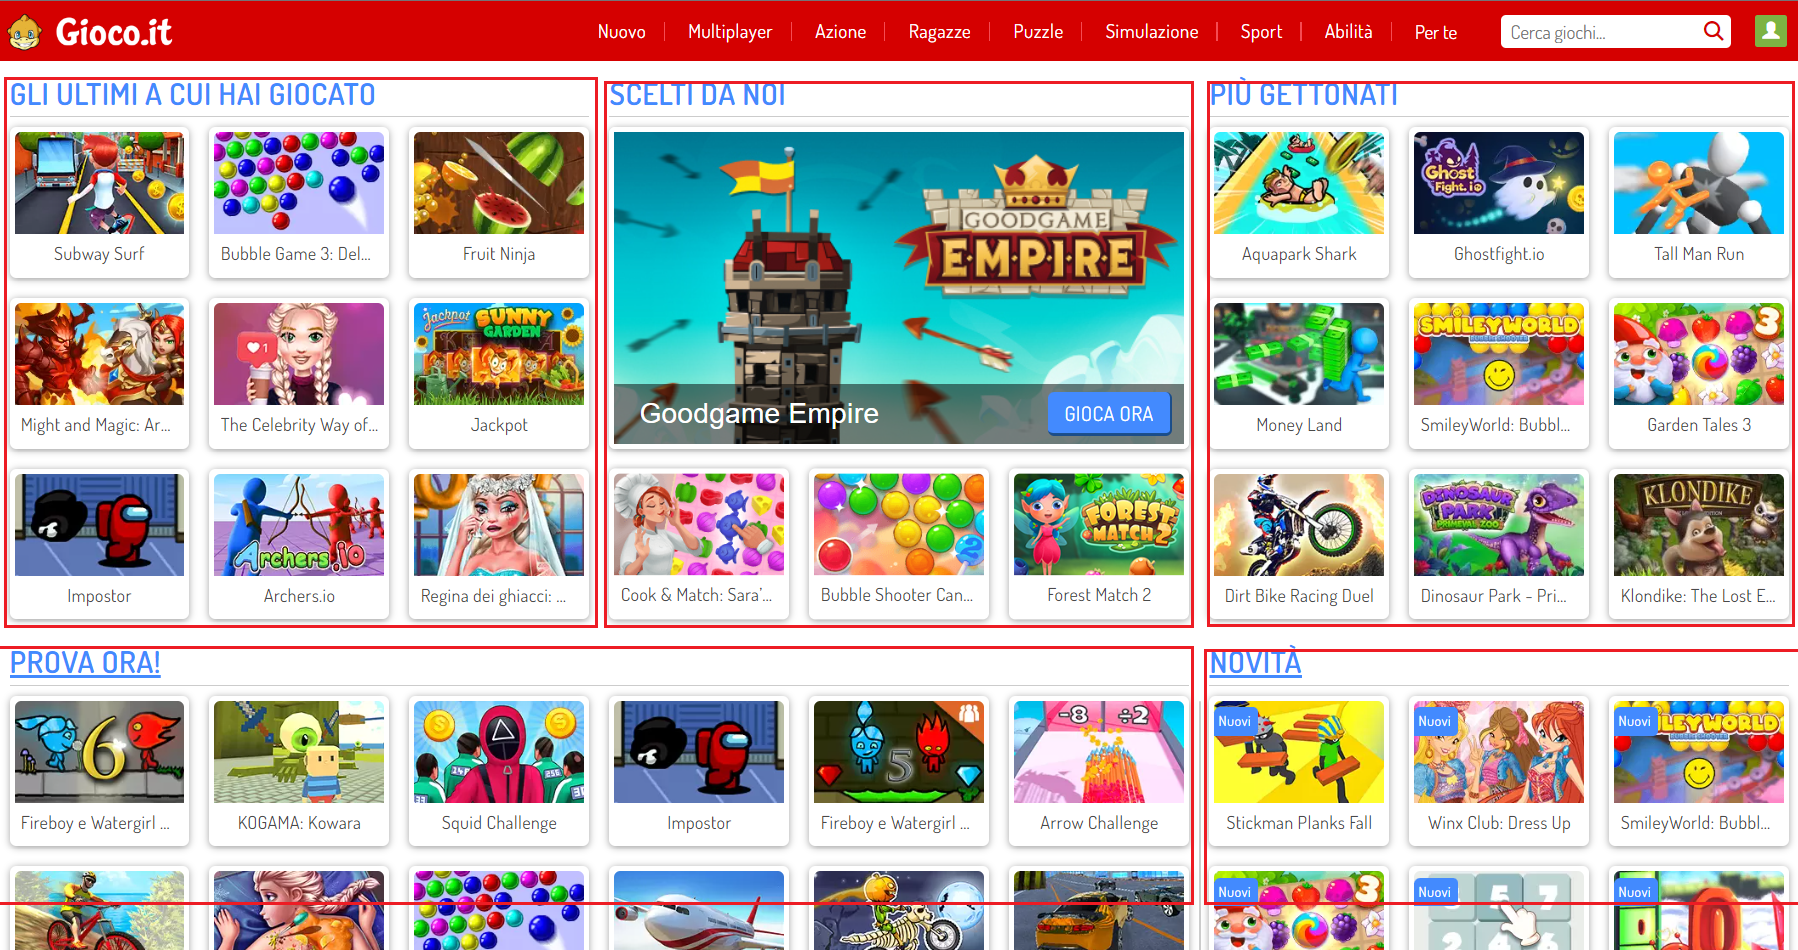
\includegraphics[width=\linewidth]{Assestment1.png}
        \centering
    \end{figure}
    \begin{figure}[H]
        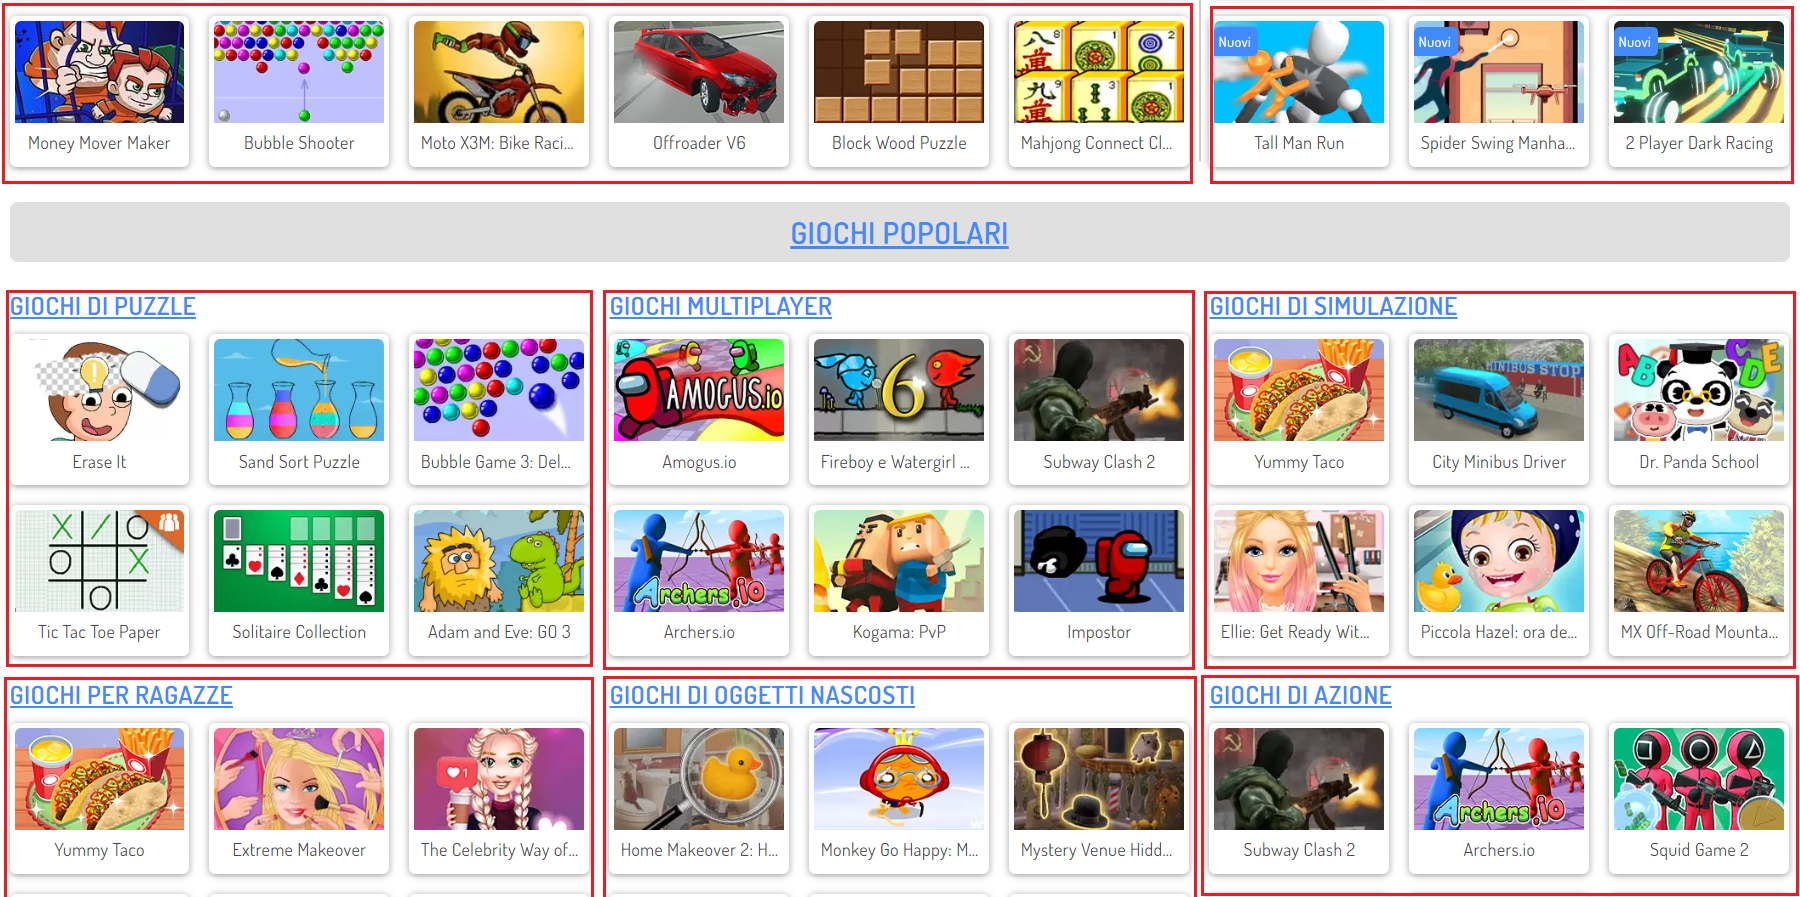
\includegraphics[width=\linewidth]{Assestment2.png}
        \centering
    \end{figure}

    Un errore visibile è che il pulsante “Nuovo” nel banner superiore della Home Page è l’unico che a differenza degli altri pur puntandolo col mouse non apre un dialog con dei giochi consigliati in quella categoria. Inoltre, cliccando le categorie su quel banner con una frequenza abbastanza alta viene aperta la pagina della lista delle categorie su una categoria diversa da quella cliccata. Le euristiche violate sono:

    \subsubsection{Home Page}
        1. \textbf{ Gli elementi della home page sono chiaramente focalizzati sui compiti chiave degli utenti (è stata evitata la "featurite")}.\\
        C’è un sovraccarico di giochi che vengono proposti all’utente, che aumentano il carico cognitivo che deve sopportare per cercare. Inoltre l’attuale divisione dello schermo rende più complicato l’orientamento da parte dell’utente poichè non è suddiviso in blocchi omogenei.\\

        3. \textbf{Le categorie dei prodotti sono presenti e chiaramente visibili nella home page}\\
        Non tutte le categorie sono visibile nella home page e non c’è un pulsante per accedere alla lista delle categorie.
\\ Non tutte le categorie sono visibile nella home page e non c’è un pulsante per accedere alla lista delle categorie.    
    \subsubsection{Navigation \& AI }
    3. \textbf{Il sistema di navigazione è broad and shallow piuttosto che deep, quindi ci sono più oggetti su un menù piuttosto che piu livelli annidati\\} 
 	Ci sono dei sottomenù evitabili. 

    \subsubsection{Page Layout e Visual Design}
    6. \textbf{Gli ipertesti sono facilmente riconoscibili senza necessità della sottolineature. }\\
    Si rende necessaria la sottolineatura degli ipertesti come nel caso di “Prova ora!” poichè hanno lo stesso font, colore e dimensione dei titoli di categoria nella prima riga che non sono però ipertesti. \\

    9. \textbf{C’è un chiaro punto di inizio visuale in ogni schermata.}\\
    Data la mancanza di coerenza nella griglia della home page risulta complesso riuscirsi correttamente ad orientare nelle varie sezioni dello schermo. Un errore comune è pensare che ad esempio la colonna 3,4,5 dei giochi della sezione “Prova ora!” siano appartenenti ad un’altra categoria, poichè la sezione “Prova ora!” è l’unica sezione lunga 6 colonne.\\

    19. \textbf{Etichette significative, colori di sfondo efficaci e uso appropriato di bordi e spazi bianchi aiutano gli utenti a identificare un insieme di elementi come un blocco funzionale discreto.}\\
	Come si può notare dalle immagini solo per separare “Prova ora!” da “Novità” viene utilizzata una leggera barra verticale grigia, non presente nella separazione di tutte le altre categorie.

    \subsubsection{Ricerca}
    Analizzeremo ora la barra di ricerca ed il suo funzionamento valutando il rispetto delle 18 euristiche di ricerca trovate. Alleghiamo uno screenshot di tre ricerche, una andata a buon fine, una che non produce risultati ed una che ritorna tanti risultati.

    \begin{figure}[H]
        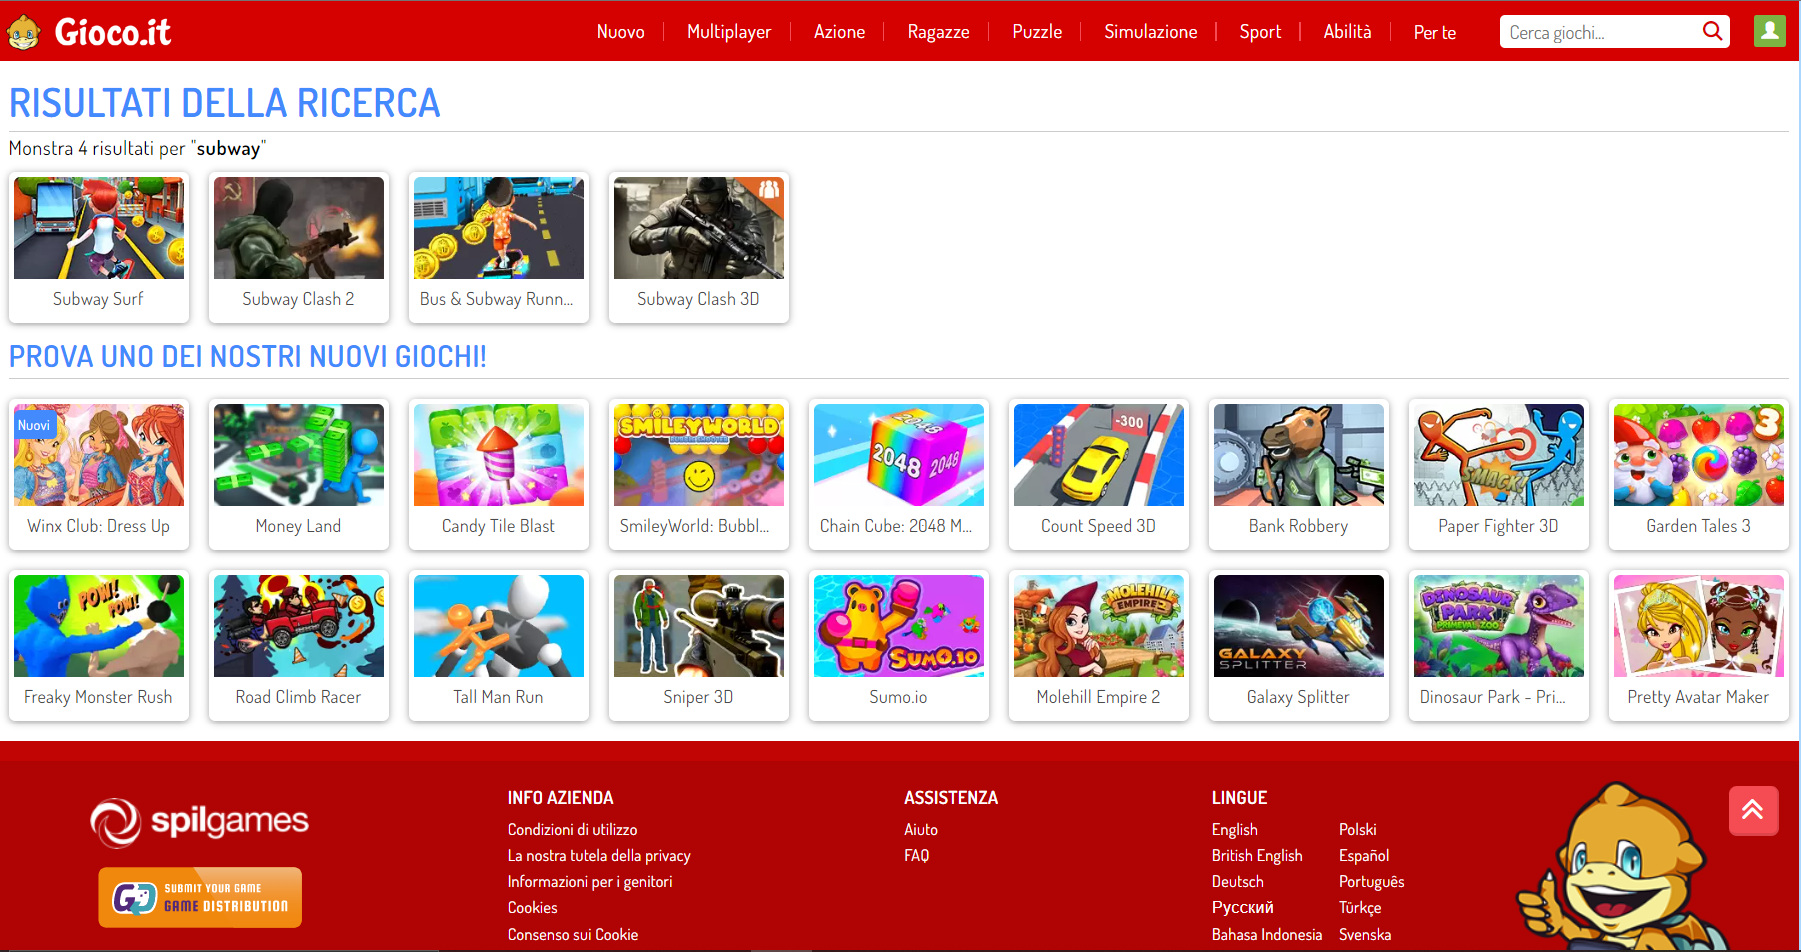
\includegraphics[width=\linewidth]{Assestment3.png}
        \centering
    \end{figure}

    \begin{figure}[H]
        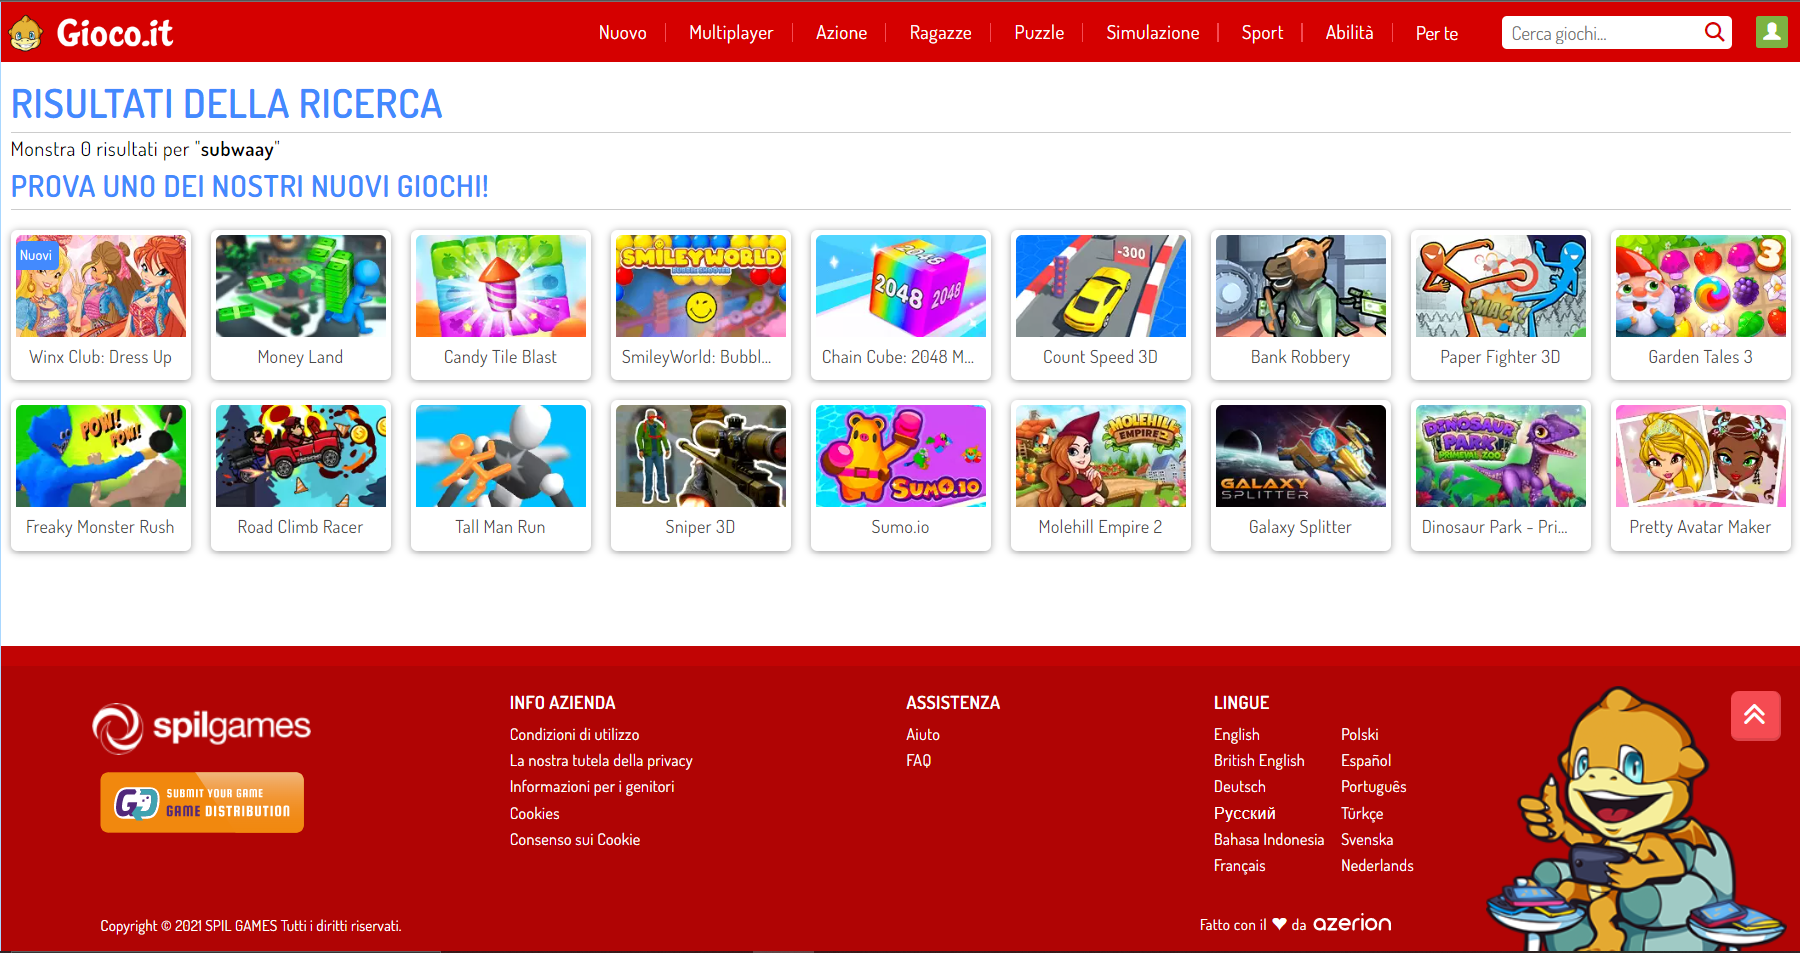
\includegraphics[width=\linewidth]{Assestment4.png}
        \centering
    \end{figure}
    \begin{figure}[H]
        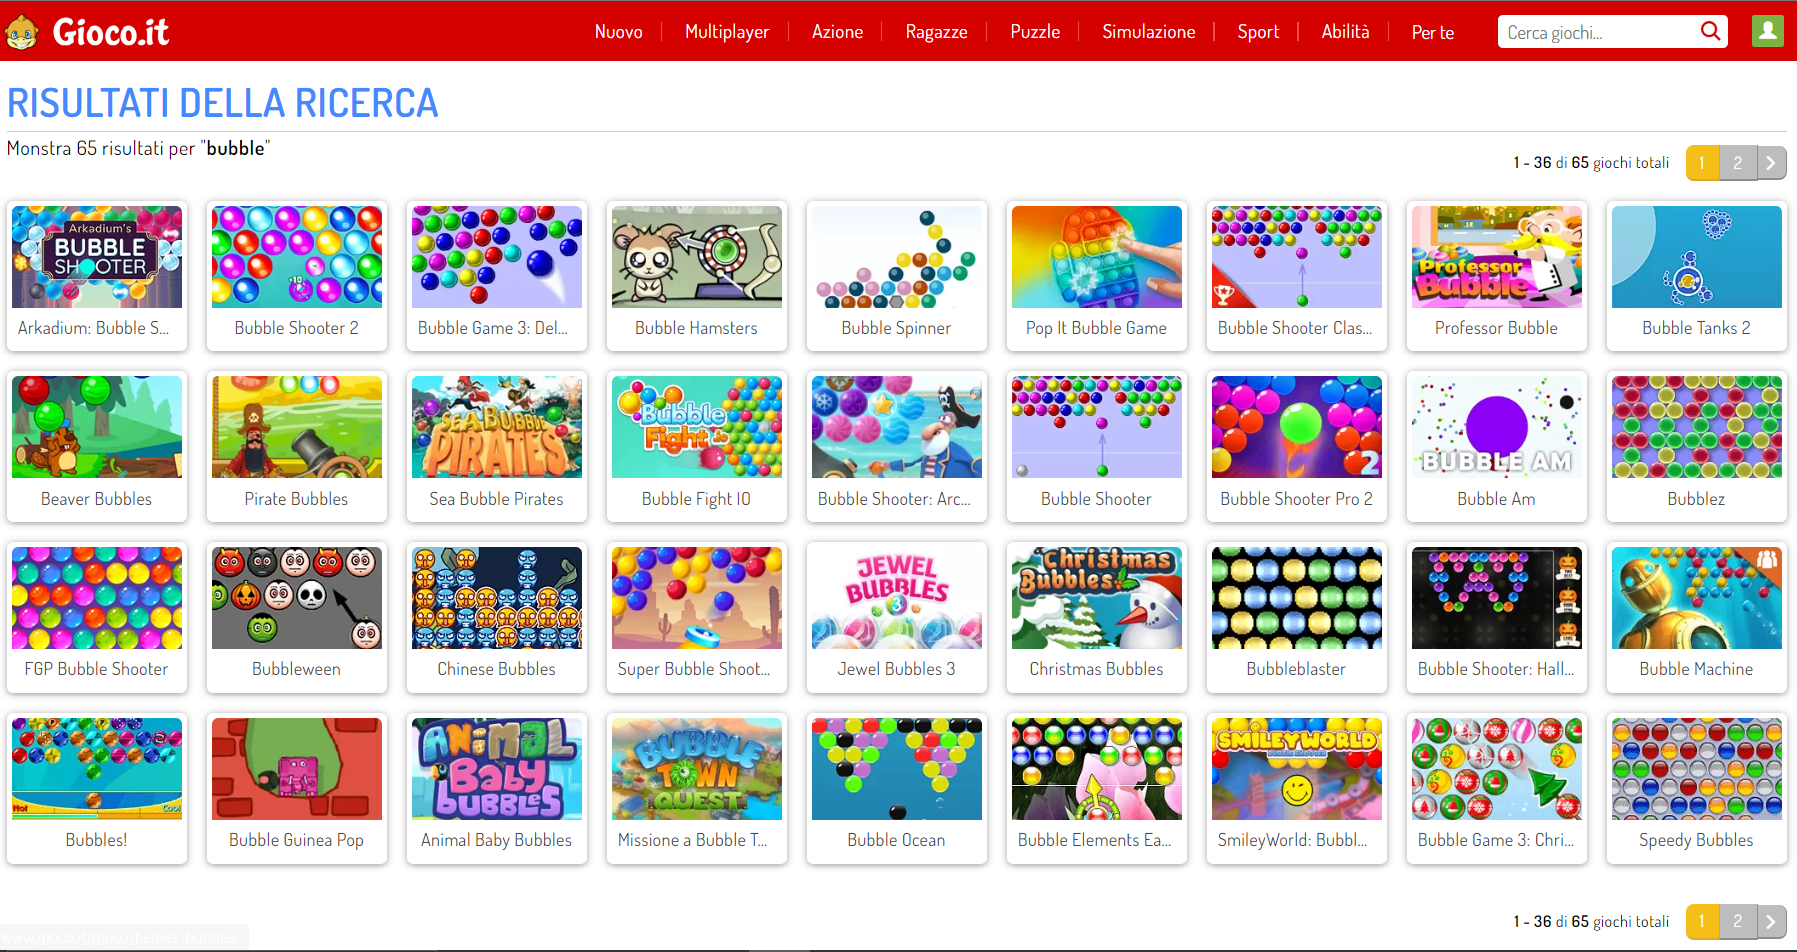
\includegraphics[width=\linewidth]{Assestment5.png}
        \centering
    \end{figure}

    4. \textbf{La ricerca dei risultati rende chiaro quanti risultati sono stati trovati ed il numero di risultati per pagine può essere modificato da parte degli utenti} \\
    Non è possibile modificare il numero di risultati per pagina\\

    5.\textbf{ Se non vengono trovati risultati il sistema offre possibili miglioramenti alla query per ritrovare informazioni }\\
    Non viene dato nessun tipo di suggerimento all’utente per migliorare la query e ottenere risultati \\

    9. \textbf{Il sistema ha un sistema di ricerca più potente che permette di raffinare le query.}\\
    Il sistema non possiede nessun tipo di motore di ricerca più potente che permette di  raffinare le query.\\
    
    16.\textbf{ I risultati della ricerca offrono delle meta informazioni.}\\
    I risultati della ricerca riportano solo nome e immagine del gioco.\\

    17. \textbf{La ricerca offre un check automatico oltre ad un controllo per plurali e sinonimi }\\
    La ricerca non offre nessun check automatico e nessun controllo per plurali e sinonimi.\\

    18.\textbf{La ricerca offre un’opzione per risultati di similarità.}\\
	La ricerca non offre opzioni per risultati di similarità.\\



    Mostriamo ora un errore 404 del sito. Come è possibile vedere il sito offre un messaggio di errore personalizzato oltre che dei consigli di giochi alternativi. 
    
    \begin{figure}[H]
        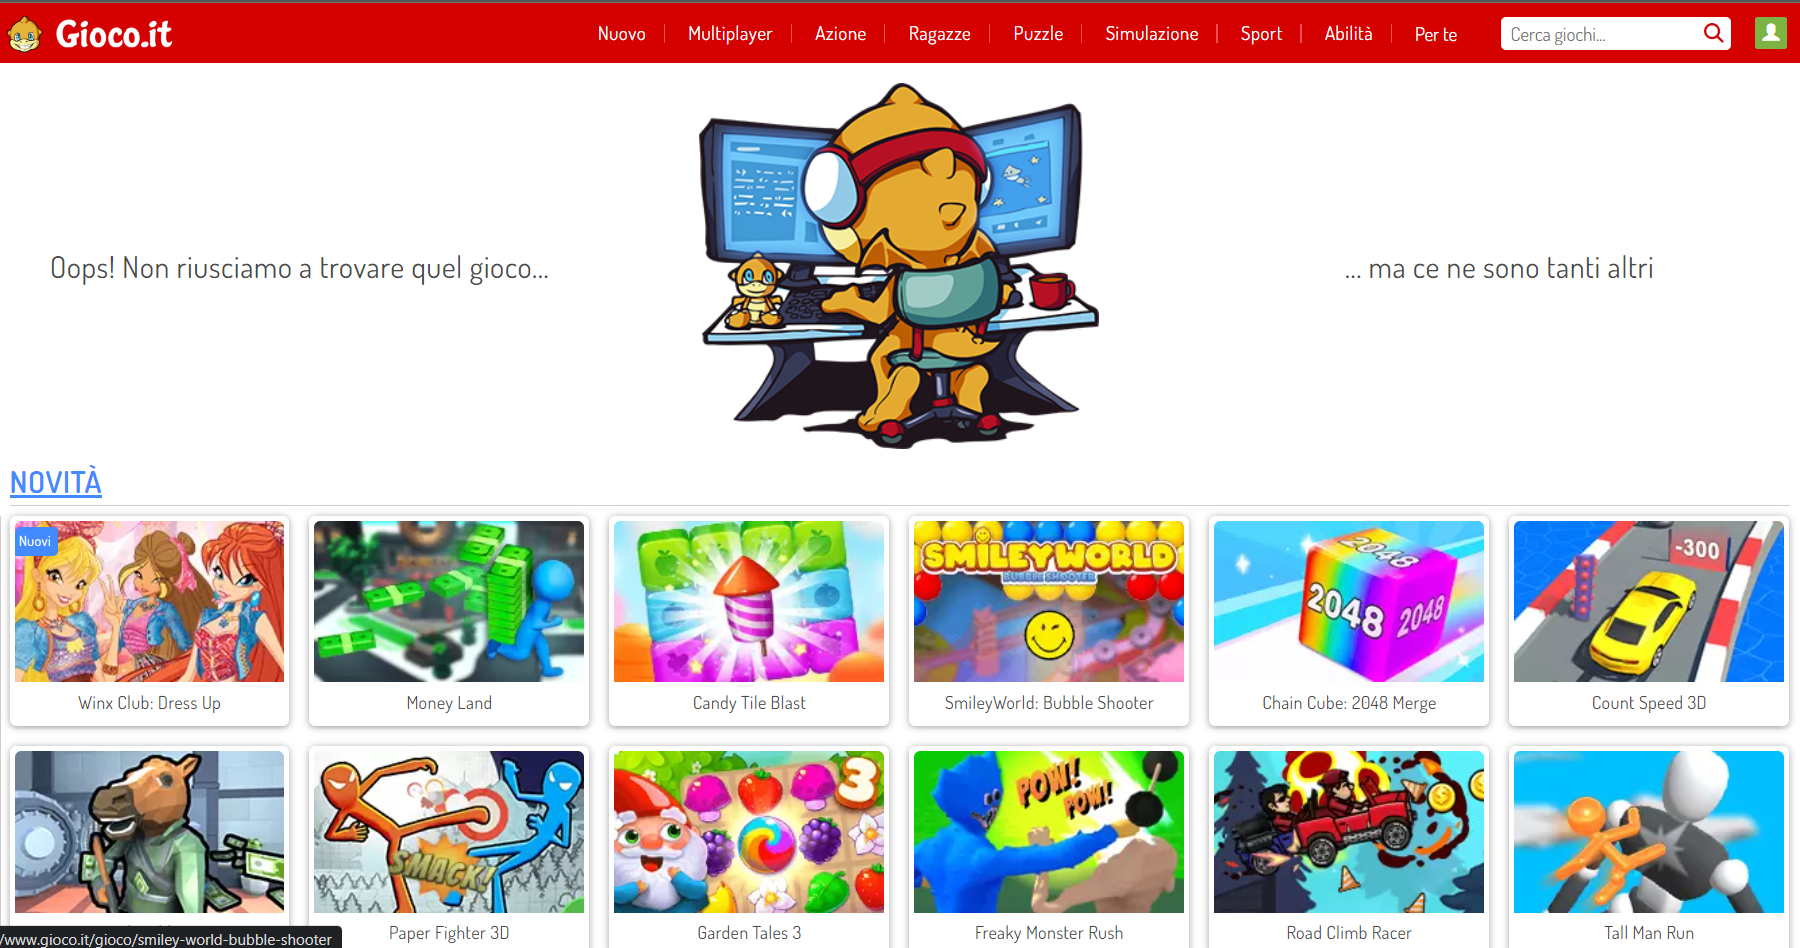
\includegraphics[width=\linewidth]{Assestment6.png}
        \centering
    \end{figure}

    \textbf{Pagina di categoria di giochi}

    \begin{figure}[H]
        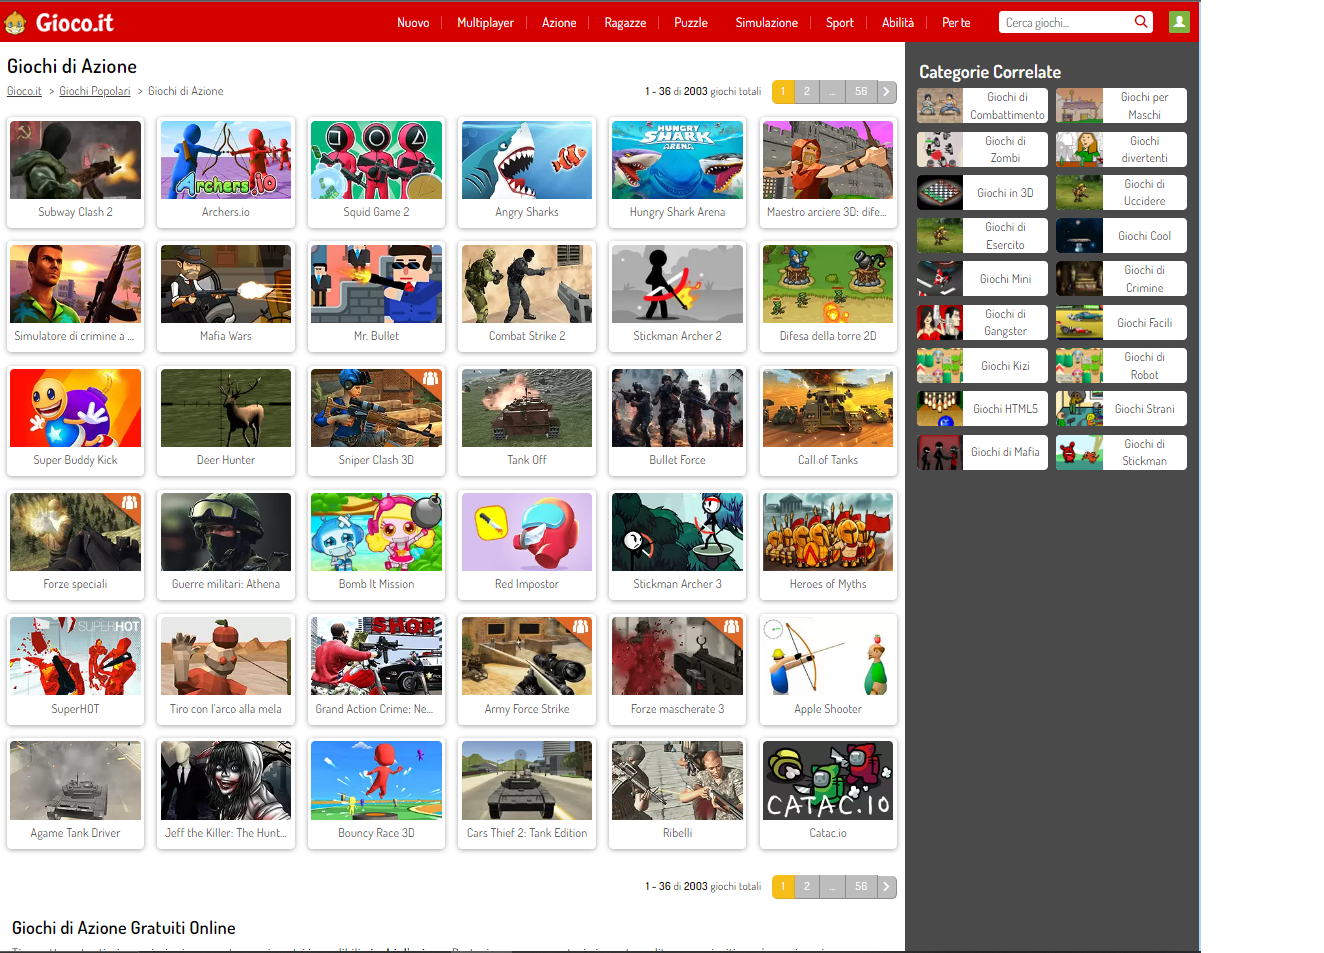
\includegraphics[width=\linewidth]{Assestment7.png}
        \centering
    \end{figure}
    

    \begin{figure}[H]
        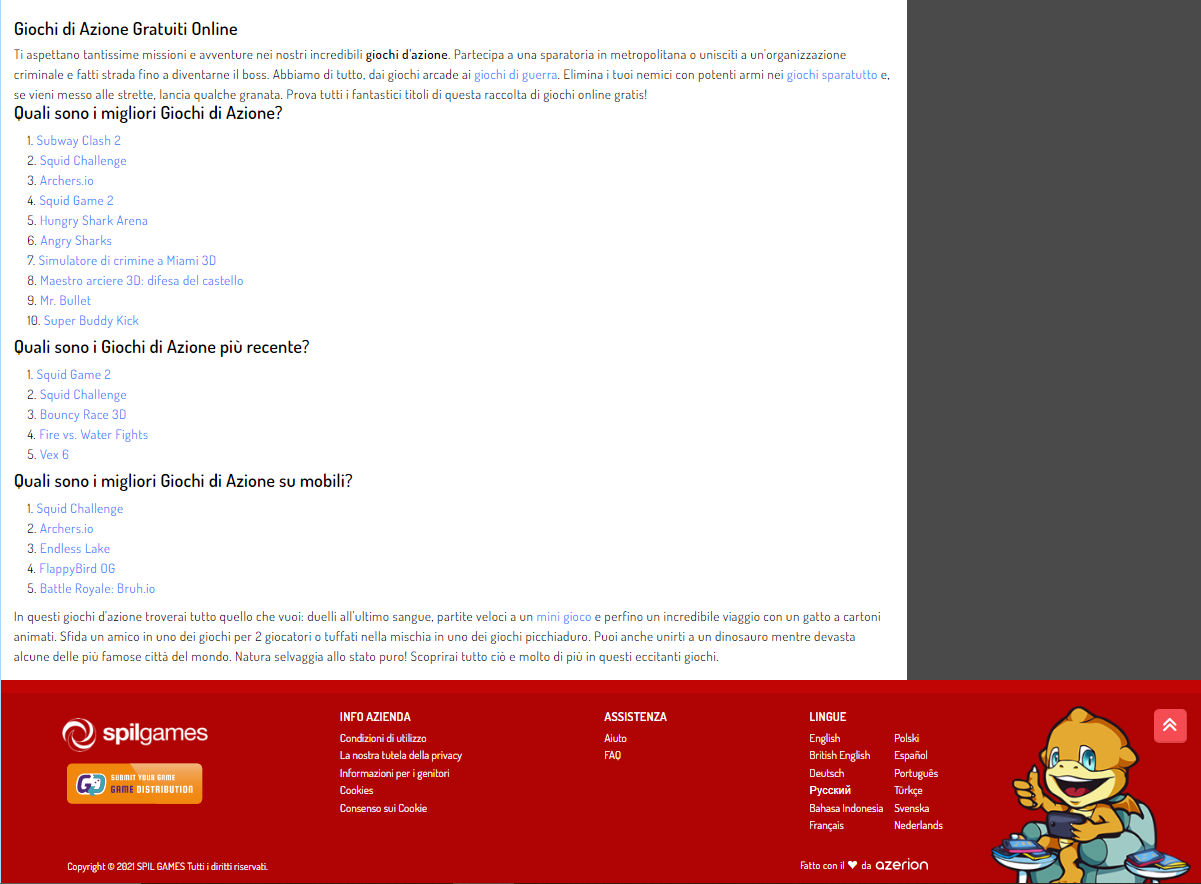
\includegraphics[width=\linewidth]{Assestment8.png}
        \centering
    \end{figure}
    La schermata presenta innanzitutto la lista di tutti i giochi, non filtrabile nè ordinabile e un testo descrittivo in basso, per il quale è necessario scrollare lo schermo. A destra inoltre vengono consigliate delle “Categorie correlate” che sono in realtà delle sottocategorie della macro-categoria di riferimento (“Azione” nel caso dello screen). Le euristiche violate in questo caso sono:

    \subsubsection{Task Orientation}
    2.\textbf{Le informazioni vengono presentate in un ordine facile e logico e naturale}\\
        Non è presente nessun tipo di ordinamento ai giochi proposti, basti notare l’ordinamento dei giochi e confrontarlo con la lista dei migliori giochi di azione elencata in basso.\\

    10.\textbf{Quando una pagina presenta tante informazioni l’utente può filtrarle} \\
        L’utente non può in nessun caso filtrare i giochi offerti da una categoria.\\
    
    \subsubsection{Navigation and IA}
    5.\textbf{Utenti possono ordinare e filtrare le pagine di categoria}\\
    Gli utenti come detto non possono filtrare in nessun modo le categorie.\\

    \subsubsection{Page Layout \& Visual Design}
    13.\textbf{Le pagine sono libere da scroll stoppers (headings o parti dello schermo che fanno credere all’utente che abbiano finito di scrollare quando non è così)}\\
    Il contenuto testuale descrittivo di ogni categoria è posto sotto la griglia dei giochi e richiede scrolling verticale. Se un utente scrolla fino all’ultima riga di giochi visualizzata e la relativa barra di spostamento tra le varie pagine (in foto in basso) potrebbe credere che non ci siano più informazioni e fermare il suo scroll.

    \begin{figure}[H]
        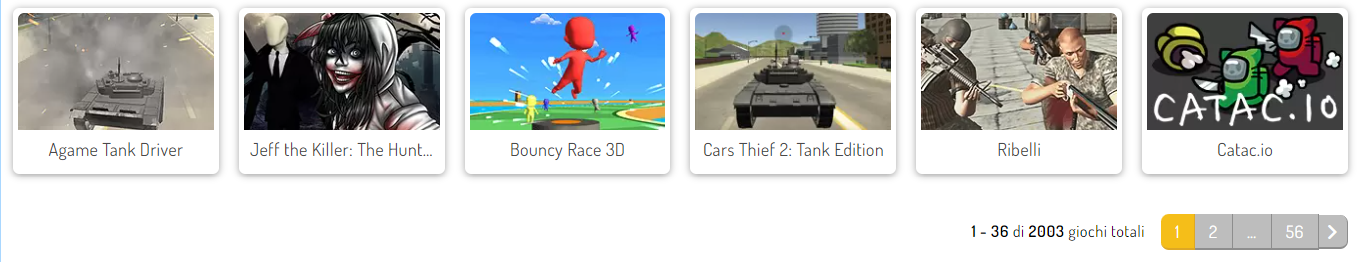
\includegraphics[width=\linewidth]{Assestment9.png}
        \centering
    \end{figure}

    16.\textbf{ Nelle pagine di contenuto le linee di testo non sono nè troppo lunghe ne troppo corte}\\
    La parte descrittiva di una categoria è spesso troppo lunga e ripetiva. Il testo potrebbe essere fortemente riassunto e si potrebbe evitare di elencare i giochi. \\

    Inoltre, per ogni categoria il sito offre una lista di sottocategorie. Non sempre però queste sotto categorie corrispondono fra loro nelle varie parti in cui è possibile accederci. Riportiamo l’esempio dei giochi di sport. 
    Il primo caso in cui si può accedere ad una lista (o un estratto della lista) dei giochi di sport è dalla home page posizionando il mouse sulla categoria sport in alto. Come si può vedere anche il nome è “Categorie Top” che non rimanda al fatto che queste siano delle sottocategorie della macro-categoria “Sport”. 
    
    \begin{figure}[H]
        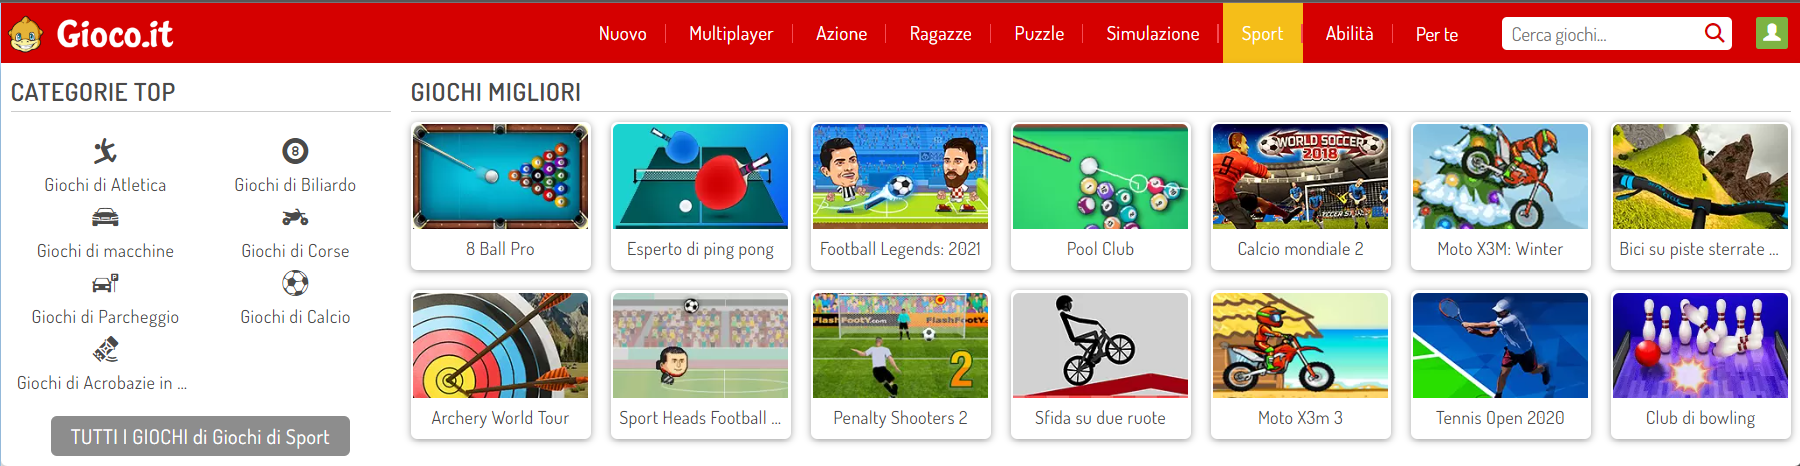
\includegraphics[width=\linewidth]{Assestment10.png}
        \centering
    \end{figure}

    Cliccando sul pulsante grigio “TUTTI I GIOCHI di Giochi di Sport” possiamo accedere al menù con la lista di tutte le sotto-categorie di ogni macro-categoria. 

    \begin{figure}[H]
        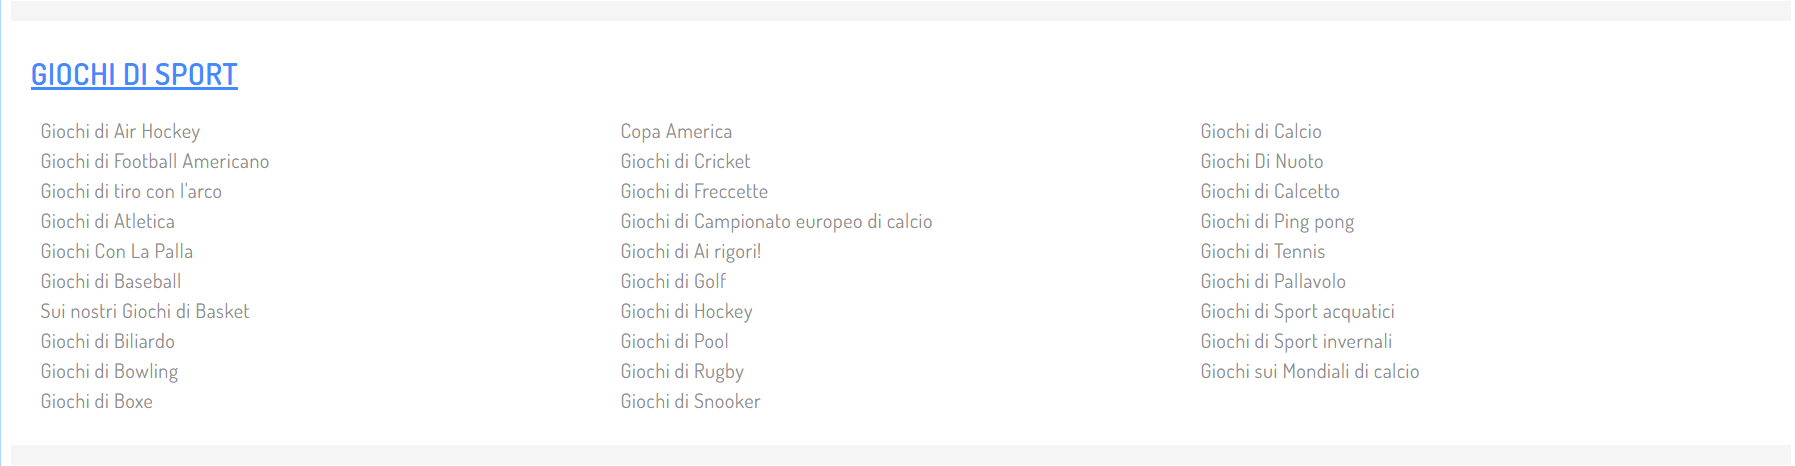
\includegraphics[width=\linewidth]{Assestment11.png}
        \centering
    \end{figure}
    \begin{wrapfigure}{r}{0.45\linewidth}
        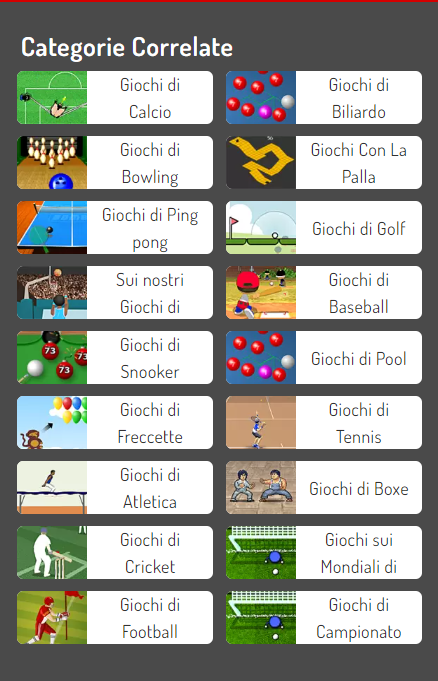
\includegraphics[width=\linewidth]{Assestment12.png}
        \centering
    \end{wrapfigure}
    Accedendo invece alla lista di tutti i giochi di Sport tramite la home page o tramite il titolo del menù con tutte le categorie e sottocategorie accediamo alla lista dei giochi di Sport vengono mostrate altre sotto-categorie, sempre mostrate con il nome “Categorie Collegate”. Come si può facilmente notare c’è una mancanza di coerenza tra le sottocategorie mostrate. Inoltre spesso, come nell’immagine qui di fianco per nomi di sottocategorie molto lunghi il nome non entra completamente nella card corrispondente lasciando incompleta la scritta.

    \newpage

    \subsubsection{Schermata di login e registrazione}
    La schermata di log in e registrazione si presenta come una schermata classica che permette l’accesso  e la registrazione tramite Facebook, Google o la classica tramite email e informazioni personali.
    Non abbiamo riscontrato violazioni o problemi. 

    \subsubsection{Profilo}
    La schermata profilo è formata da ulteriori sottomenù.

    \begin{figure}[H]
        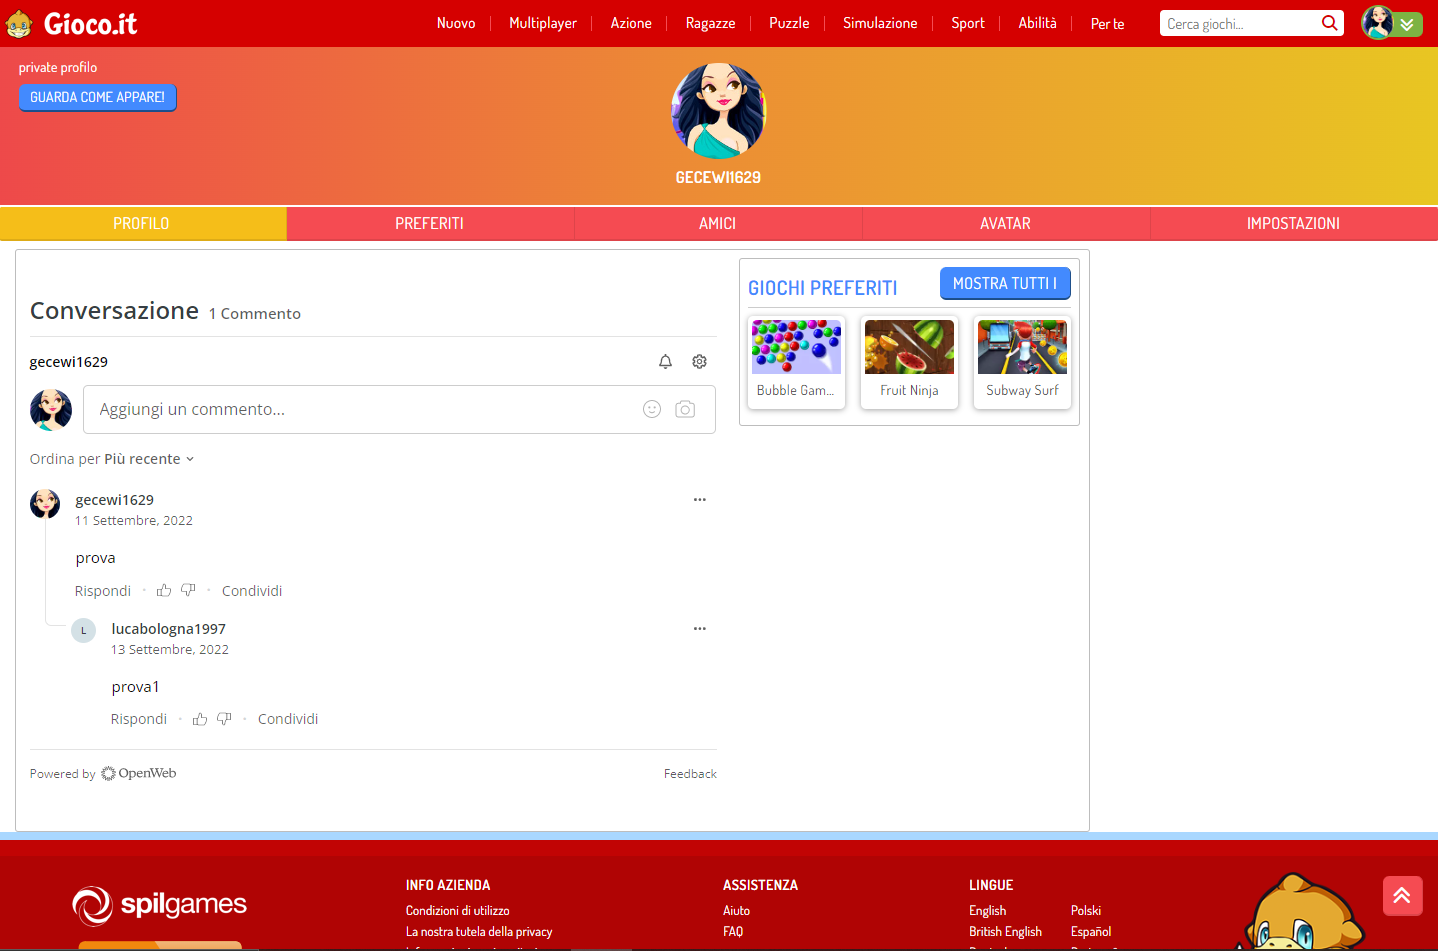
\includegraphics[width=\linewidth]{Assestment13.png}
        \centering
    \end{figure}

    \begin{figure}[H]
        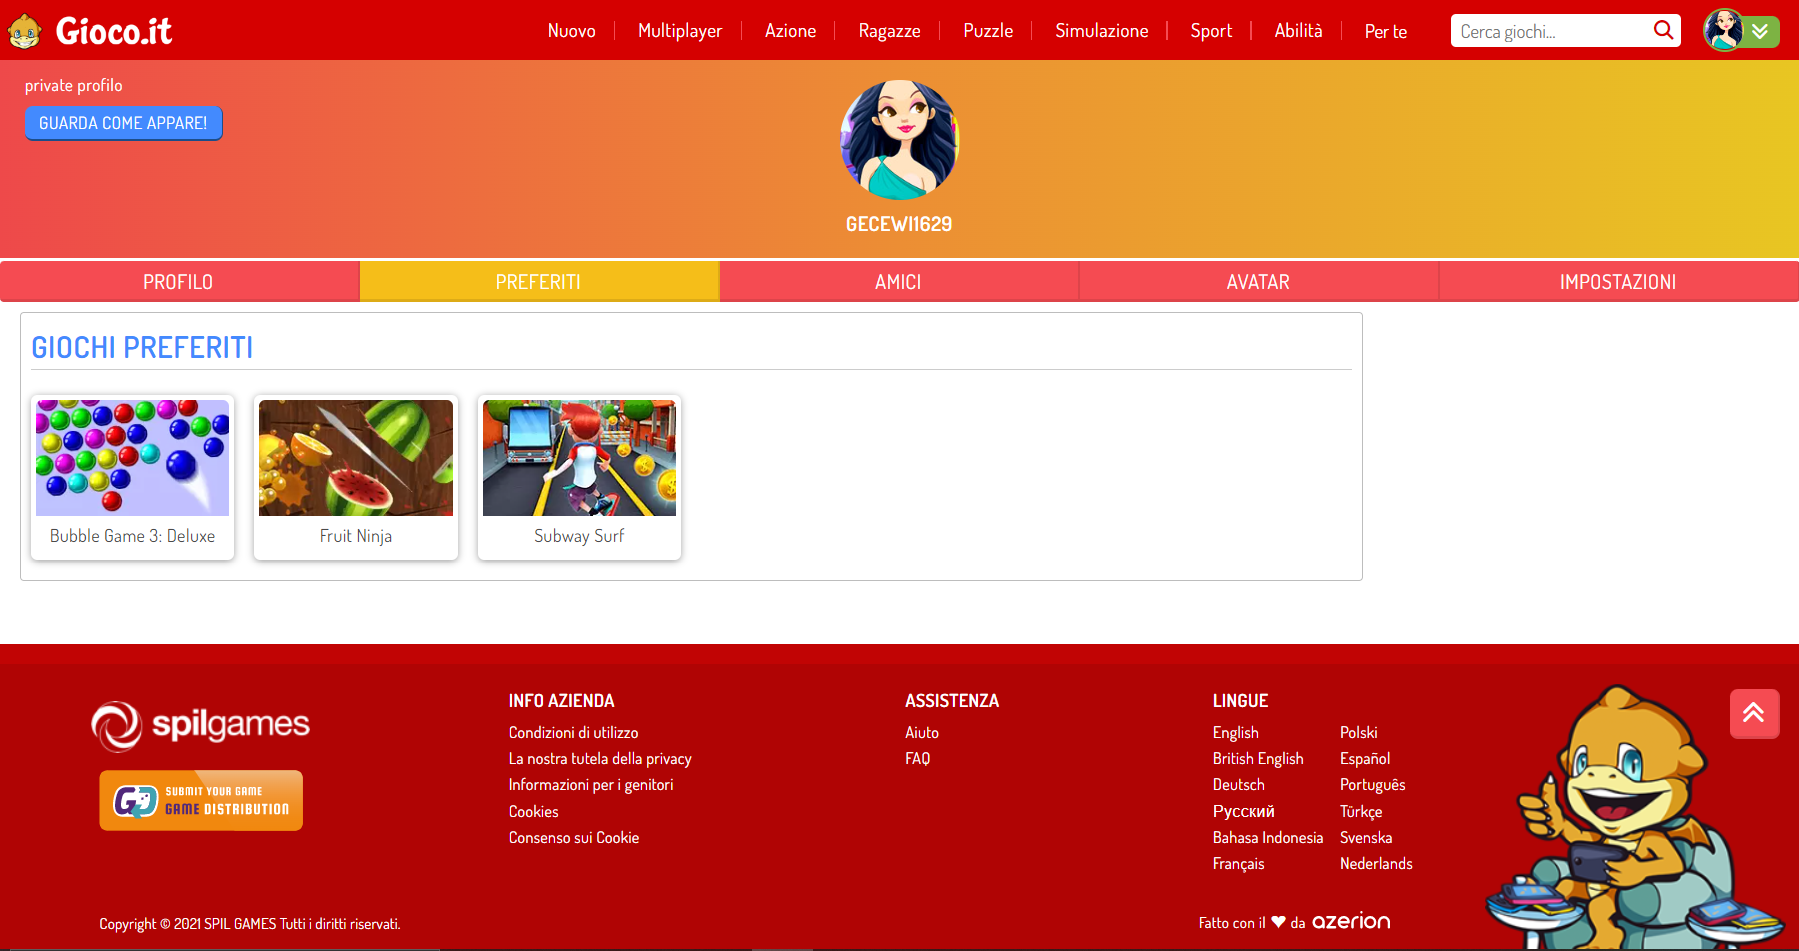
\includegraphics[width=\linewidth]{Assestment14.png}
        \centering
    \end{figure}
    Questa sezione del menù comprende l’immagine del profilo, un bottone che permette di visualizzare come il nostro profilo appare ad altri utenti poi un menù formato da cinque tab che permettono di spostarsi all’interno di tutte le aree del profilo. Infine la sezione profilo contiene una sezione nella quale è possibile ricevere e rispondere a commenti con degli amici. Questa sezione viene spesso sostituita da un messaggio di errore. Poi c’è un link ai giochi preferiti dell’utente, accessibili anche tramite il tasto sui tab. \\
    Le violazioni commesse in questo caso sono: \\

    \subsubsection{Task Orientation}
    1.\textbf{Il sito è libero da informazioni irrilevanti e che possono generare confusione}\\
        C'è una ripetizione dei giochi preferiti, presenti e accessibili sia da questa sezione che dal tab preferiti. Inoltre la sezione commenti potrebbe essere confusionaria e irrilevante siccome non è presente un'organizzazione dei commenti.\\

    \begin{figure}[H]
        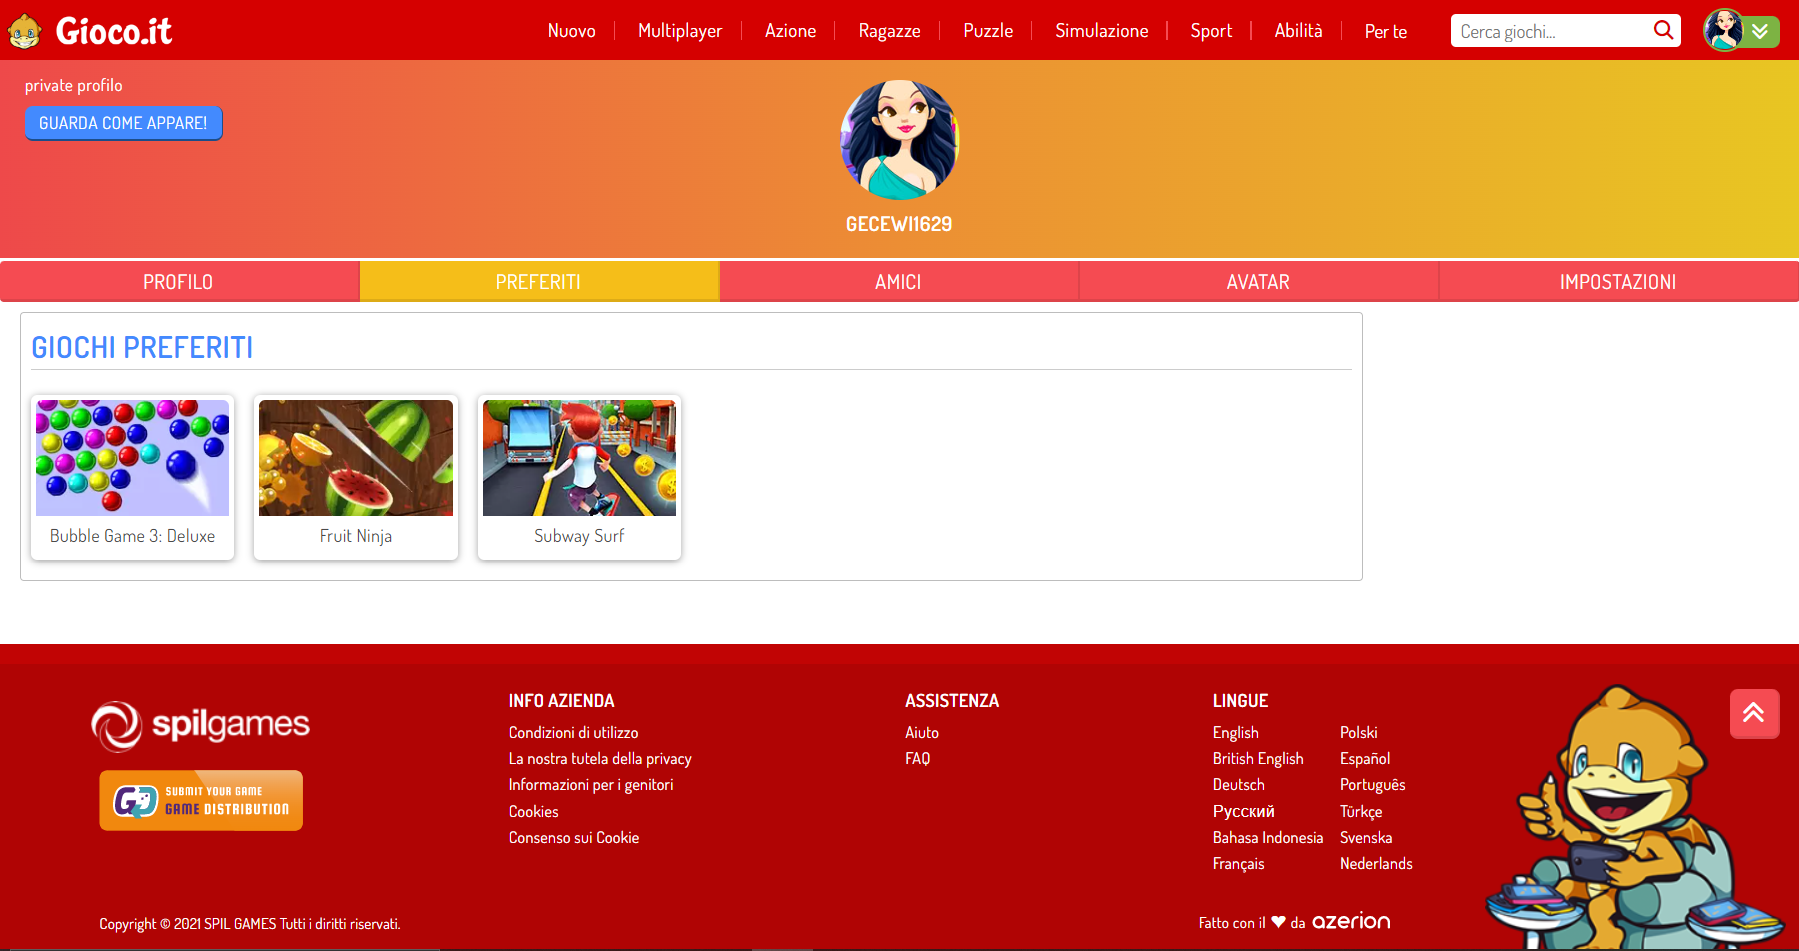
\includegraphics[width=\linewidth]{Assestment14.png}
        \centering
    \end{figure}

    La sezione dei preferiti contiene invece solo la lista dei giochi preferiti. E’ possibile accedervi ed eliminarli dalla lista. Non abbiamo riscontrato delle violazioni in questa parte.

    \begin{figure}[H]
        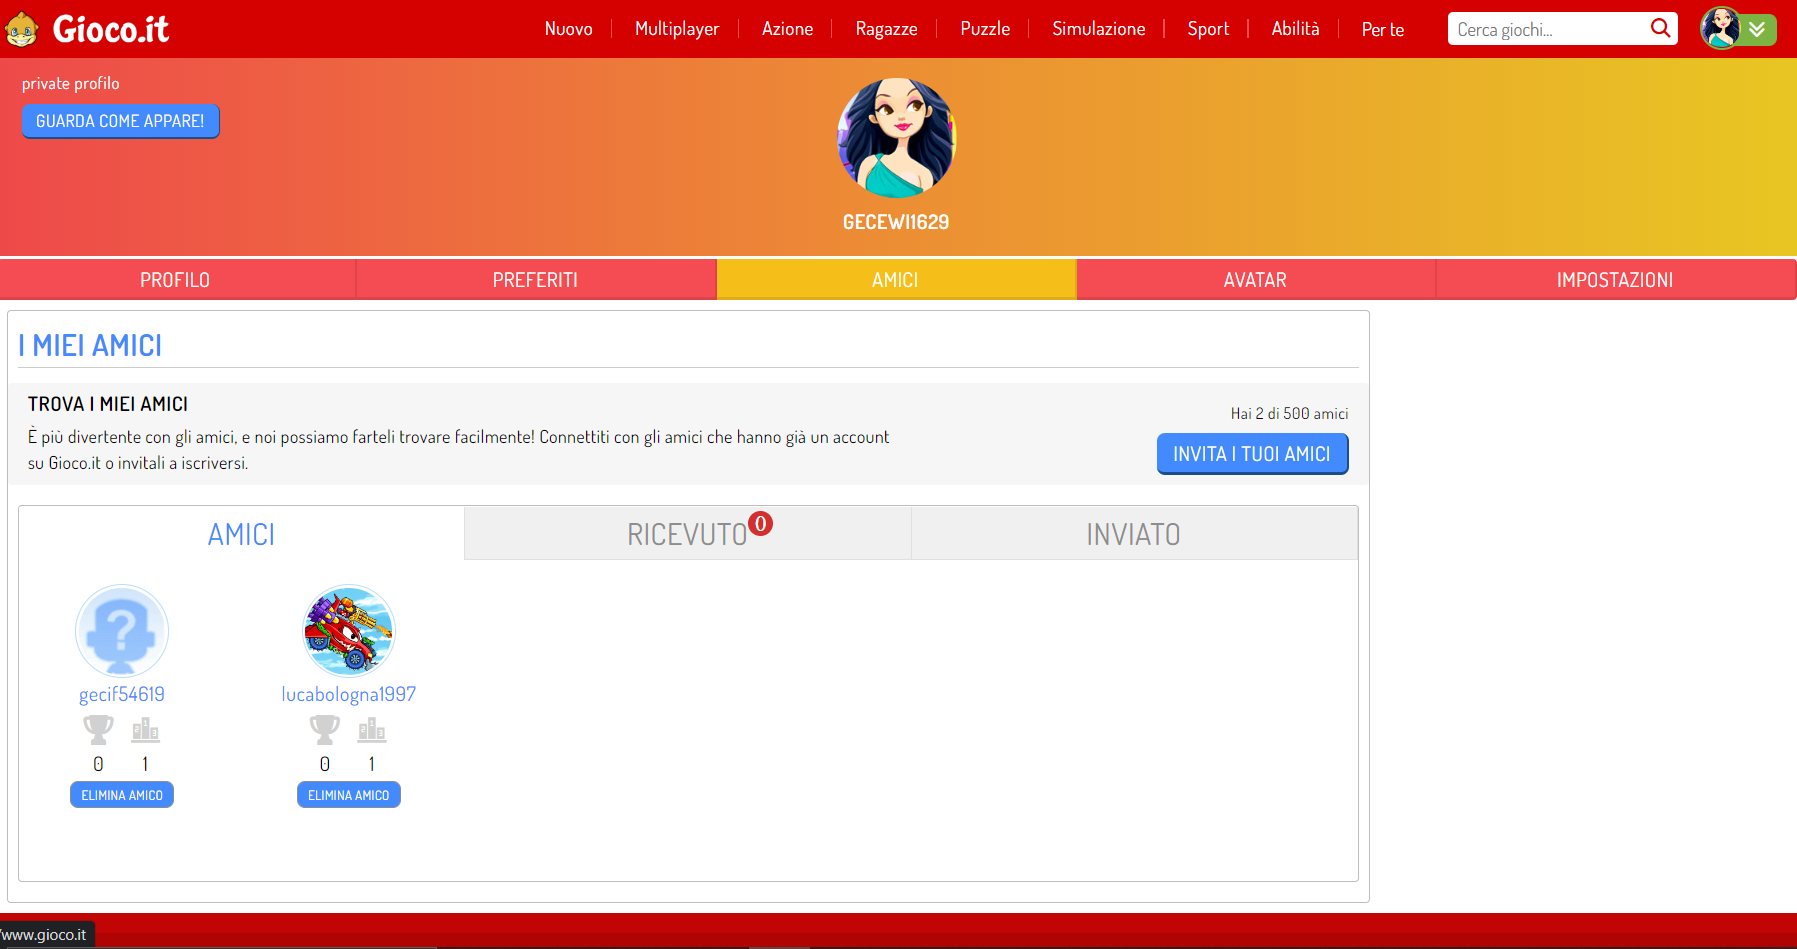
\includegraphics[width=\linewidth]{Assestment15.png}
        \centering
    \end{figure}

    La sezione amici si divide in tre sotto tabs, nelle quali è possibile vedere la lista di amici, le richieste di amicizia inviate e quelle ricevute. Inoltre permette con un semplice bottone di inviare delle richieste di amicizia. Anche in questo caso non abbiamo trovato delle violazioni. 

    \begin{figure}[H]
        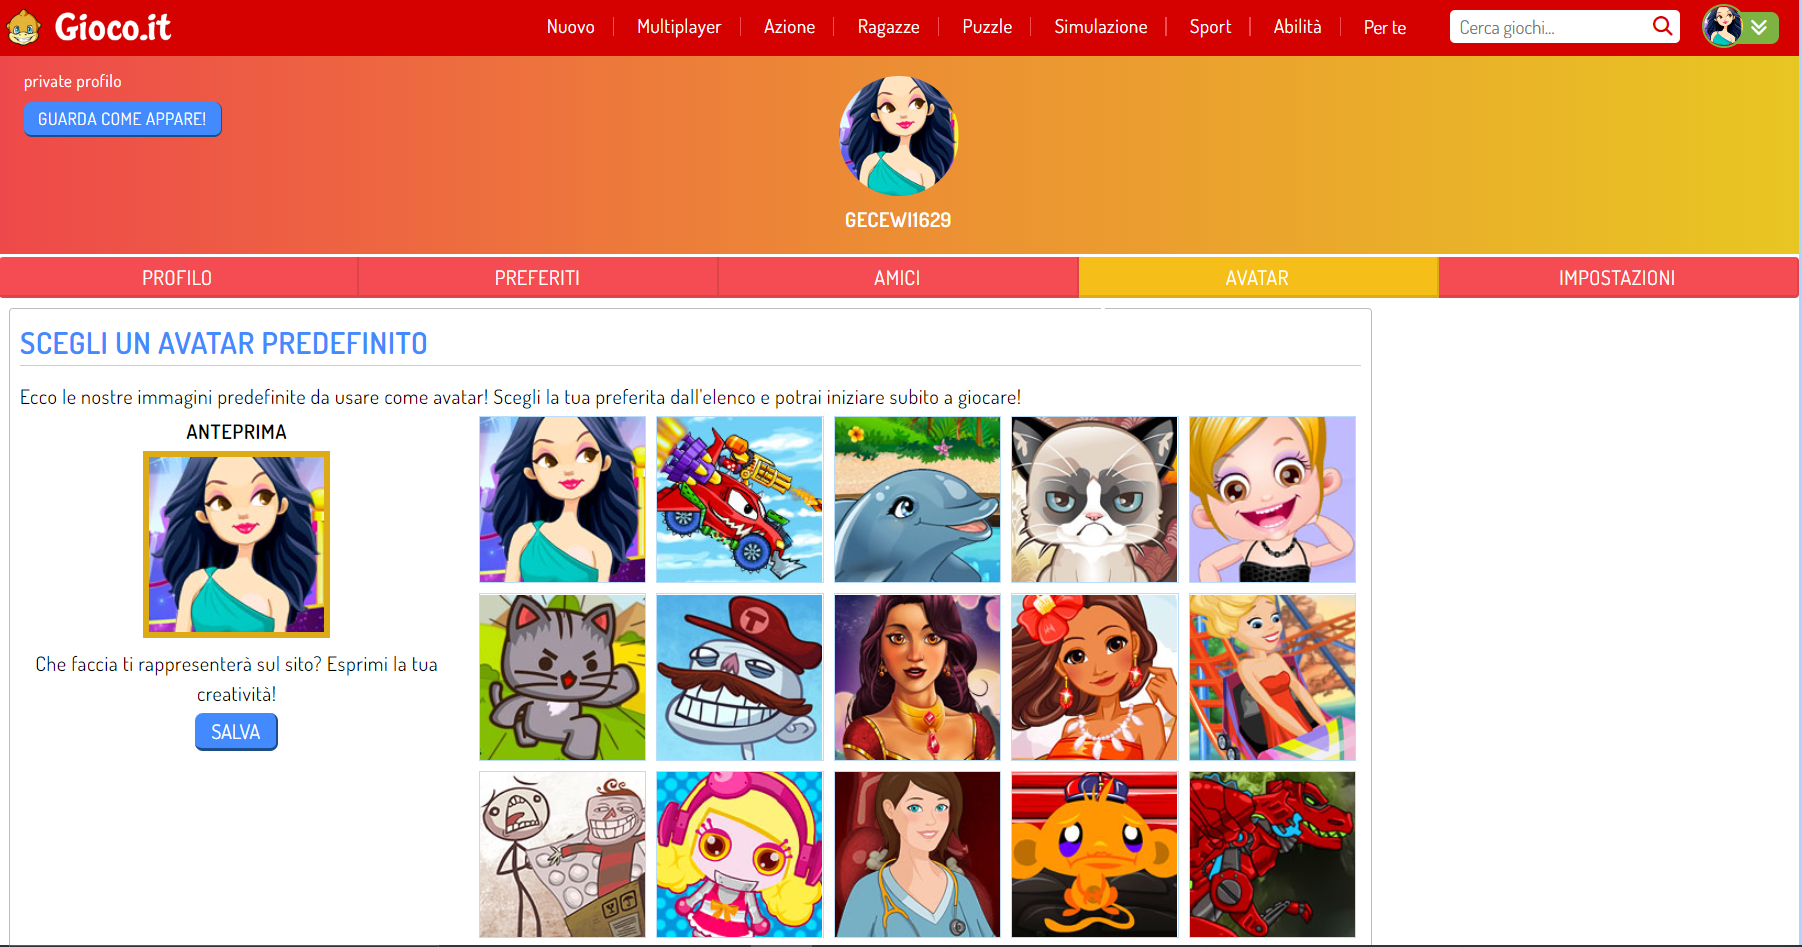
\includegraphics[width=\linewidth]{Assestment16.png}
        \centering
    \end{figure}

    La schermata avatar invece permette di modificare l’avatar dell’account con degli avatar preimpostati del sito. Anche in questo caso non abbiamo trovato delle importanti violazioni. Non è però possibile rimuovere l’immagine del profilo dopo averne messo una (tornando quindi ad un account senza avatar) e non è possibile caricare un’immagine del profilo a proprio piacimento. 

    \begin{figure}[H]
        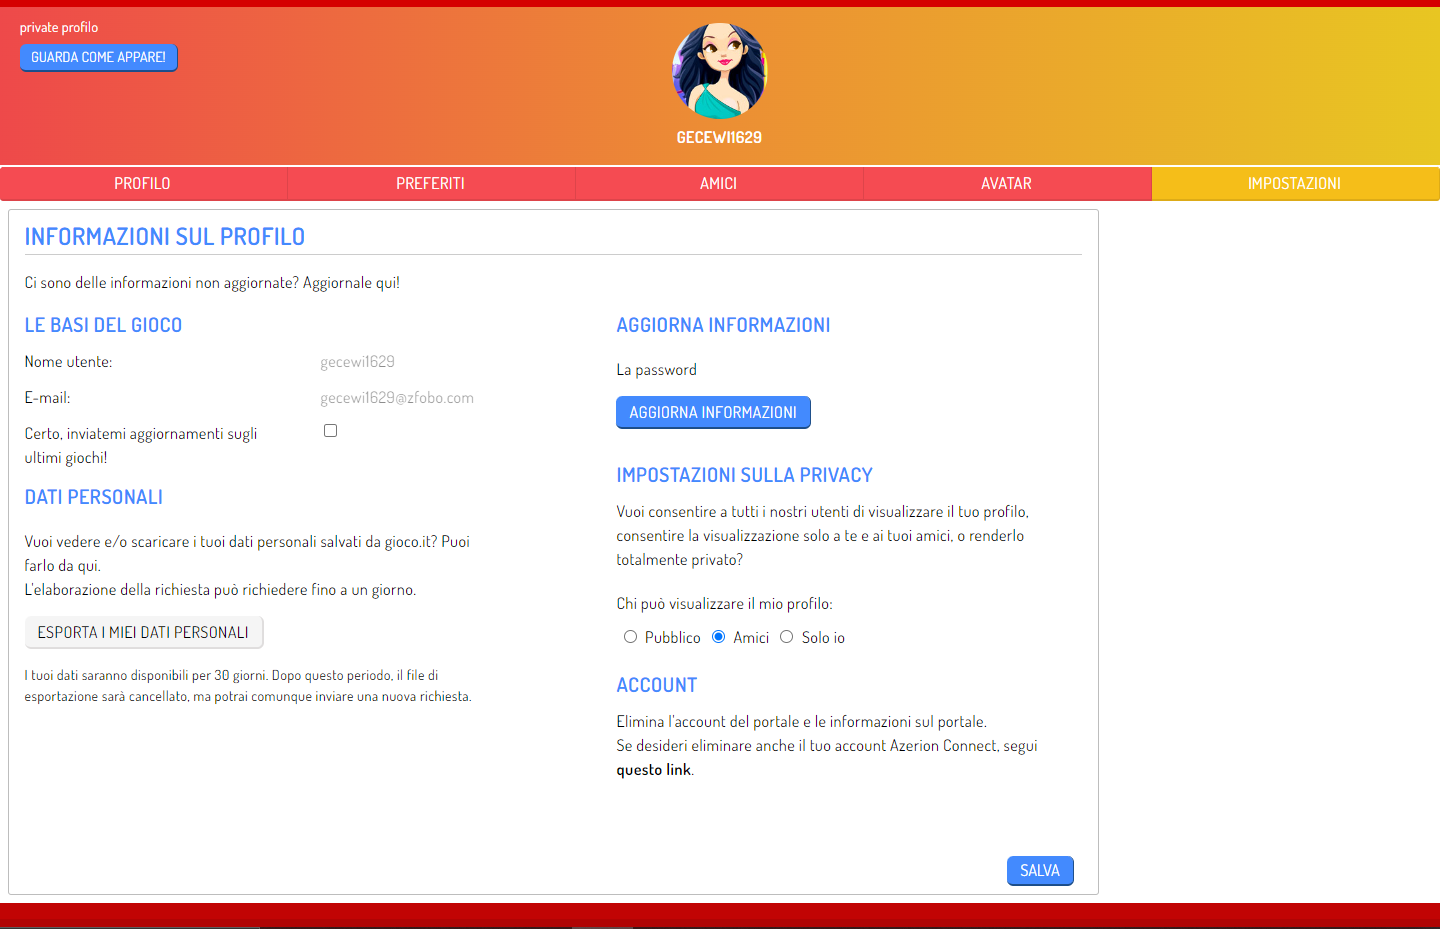
\includegraphics[width=\linewidth]{Assestment17.png}
        \centering
    \end{figure}

    Per quanto riguarda la sezione impostazioni possiamo trovare delle violazioni.
    Innanzitutto la sezione “Aggiorna Informazioni” si riferisce solo all’aggiornamento della password, il titolo può essere quindi motivo di confusione negli utenti. La scritta inoltre “La password” è totalmente inutile poichè non c’è nessun modo di visionare la password.
    Le violazioni sono:

    \subsubsection{Task Orientation}
    1.\textbf{Il sito è libero da informazioni irrilevanti e che possono generare confusione}\\
	Pensiamo alla scritta “La password” che potrebbe confondere gli utenti o alla scritta “Aggiorna informazioni”.\\
    
    11.\textbf{  Il sito permette agli utenti di customizzare dei parametri di tempo operazionali (tempo di logoff, tempo d’uso ecc)}\\
    Il sito non permette di modificare nessun tipo di parametro operazionale. \\

    \subsubsection{FAQ \& HELP}
    \begin{figure}[H]
        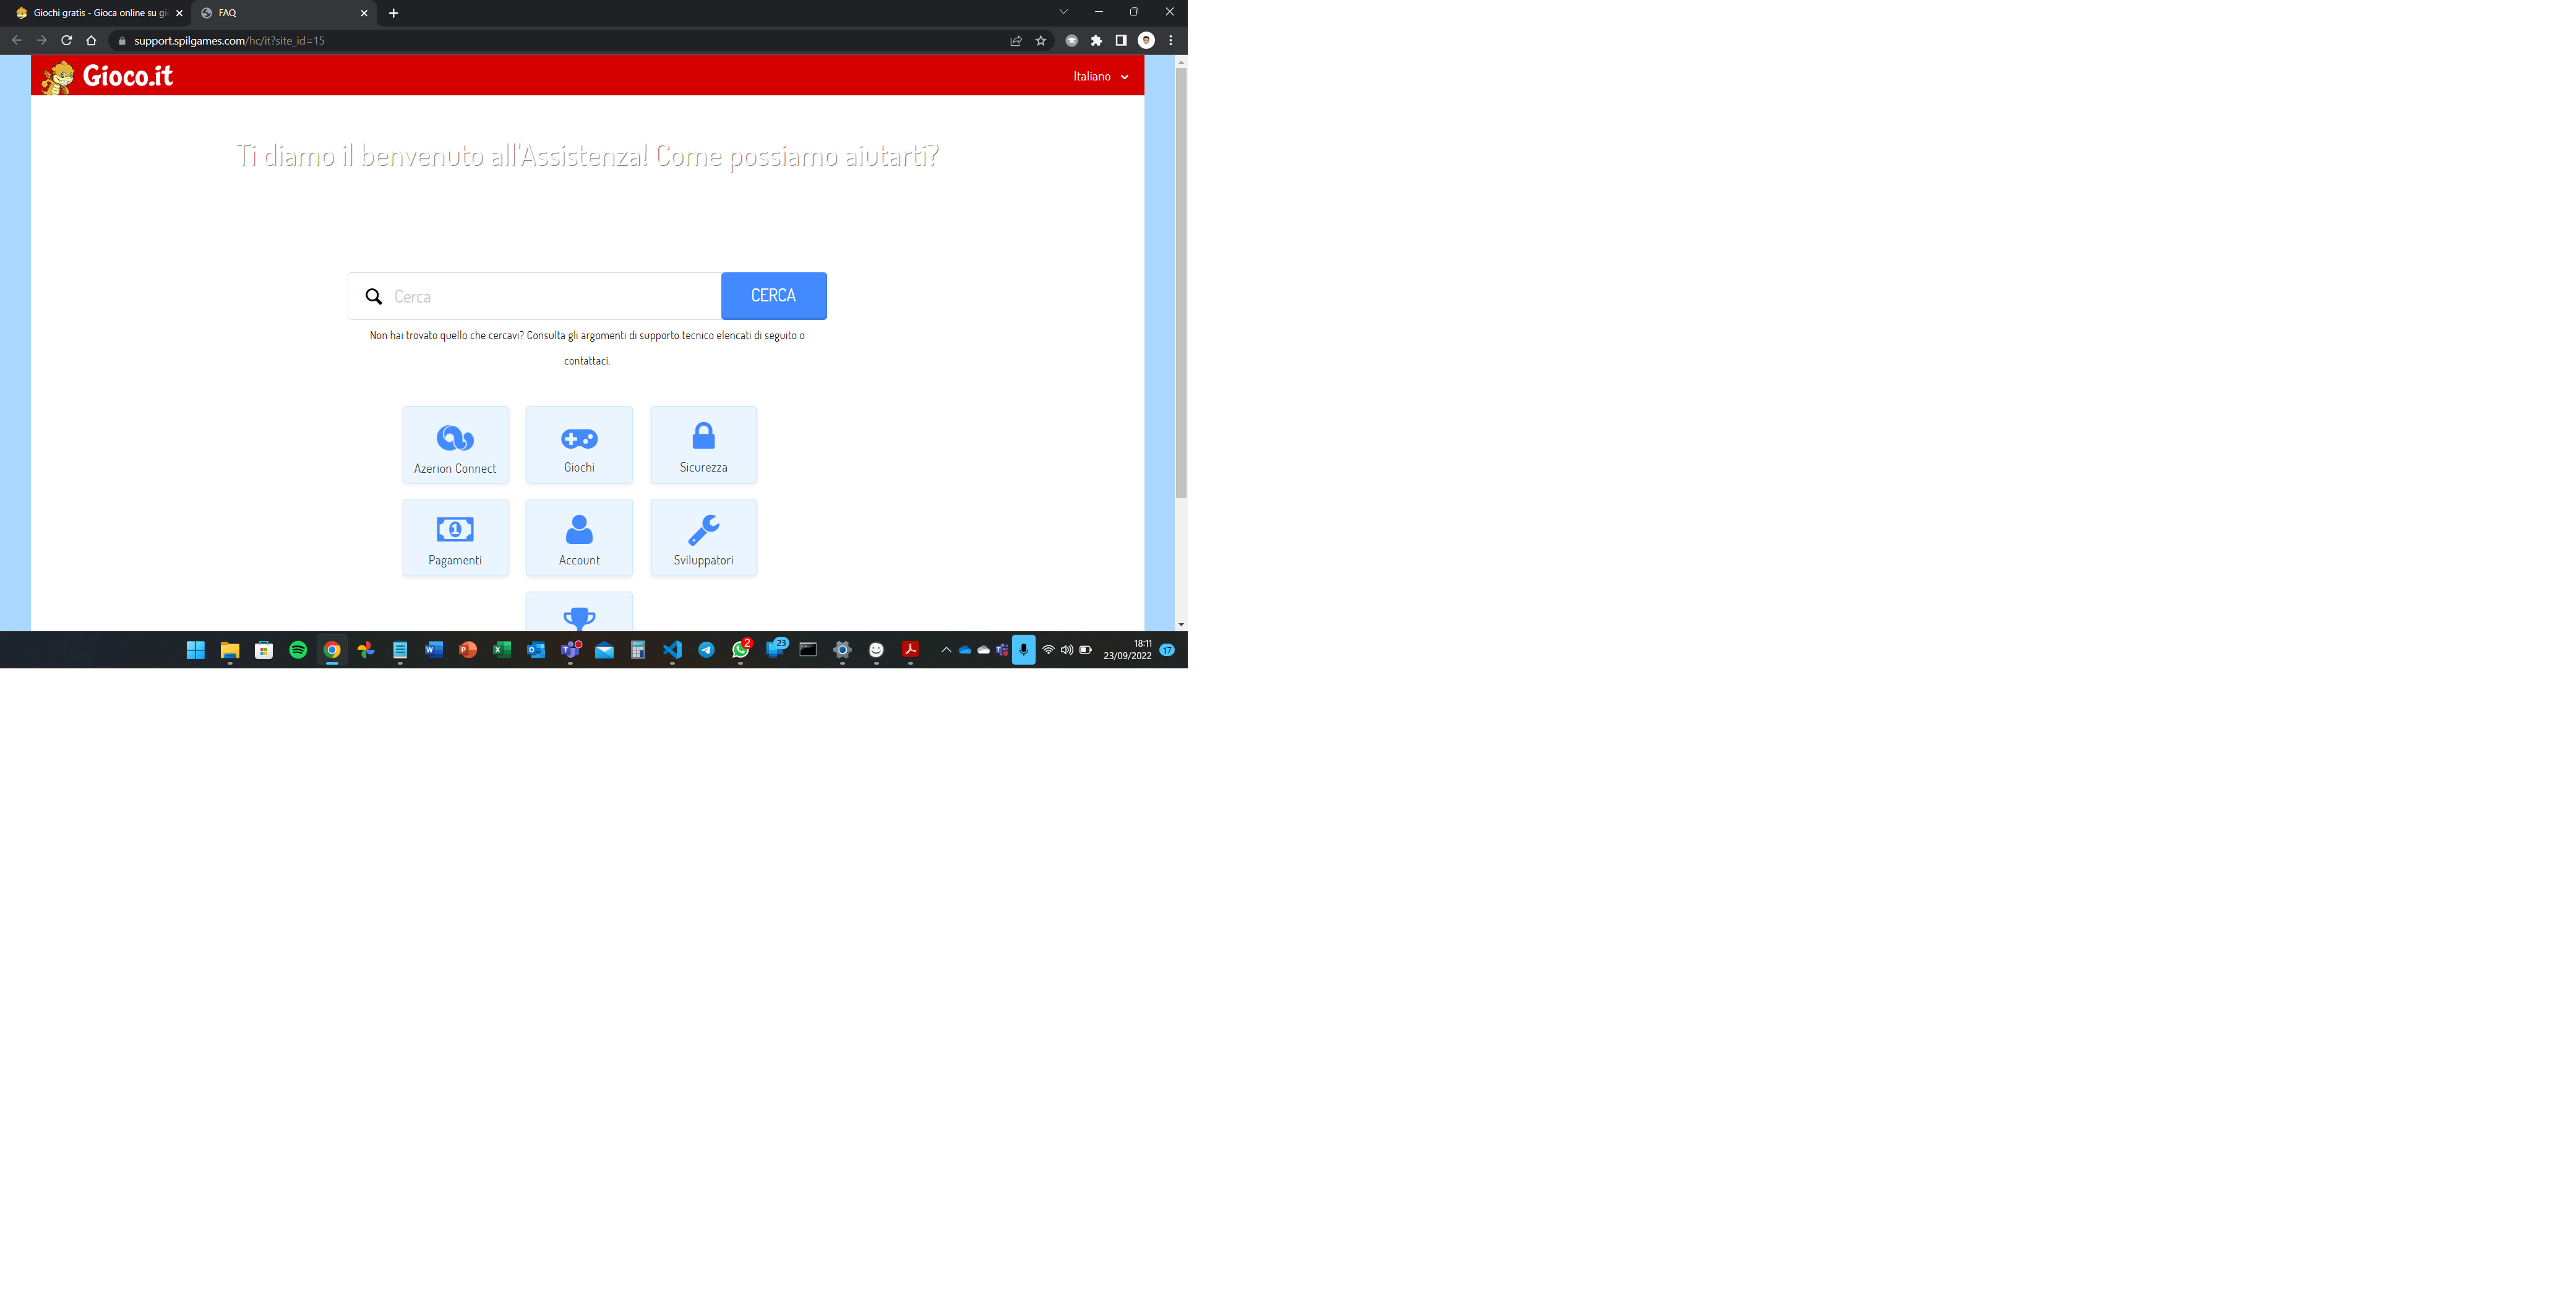
\includegraphics[width=\textwidth]{Assestment20.png}
        \centering
    \end{figure}
    Questa è la schermata dell'Aiuto di Gioco.it. Viene presentata una schermata divisa in varie sezioni in base agli argomenti. Accedendo ad ognuna si queste sezioni si viene reindirizzati in una pagina contentente una lista di domande per quel determinato argomento. 
    \begin{figure}[H]
        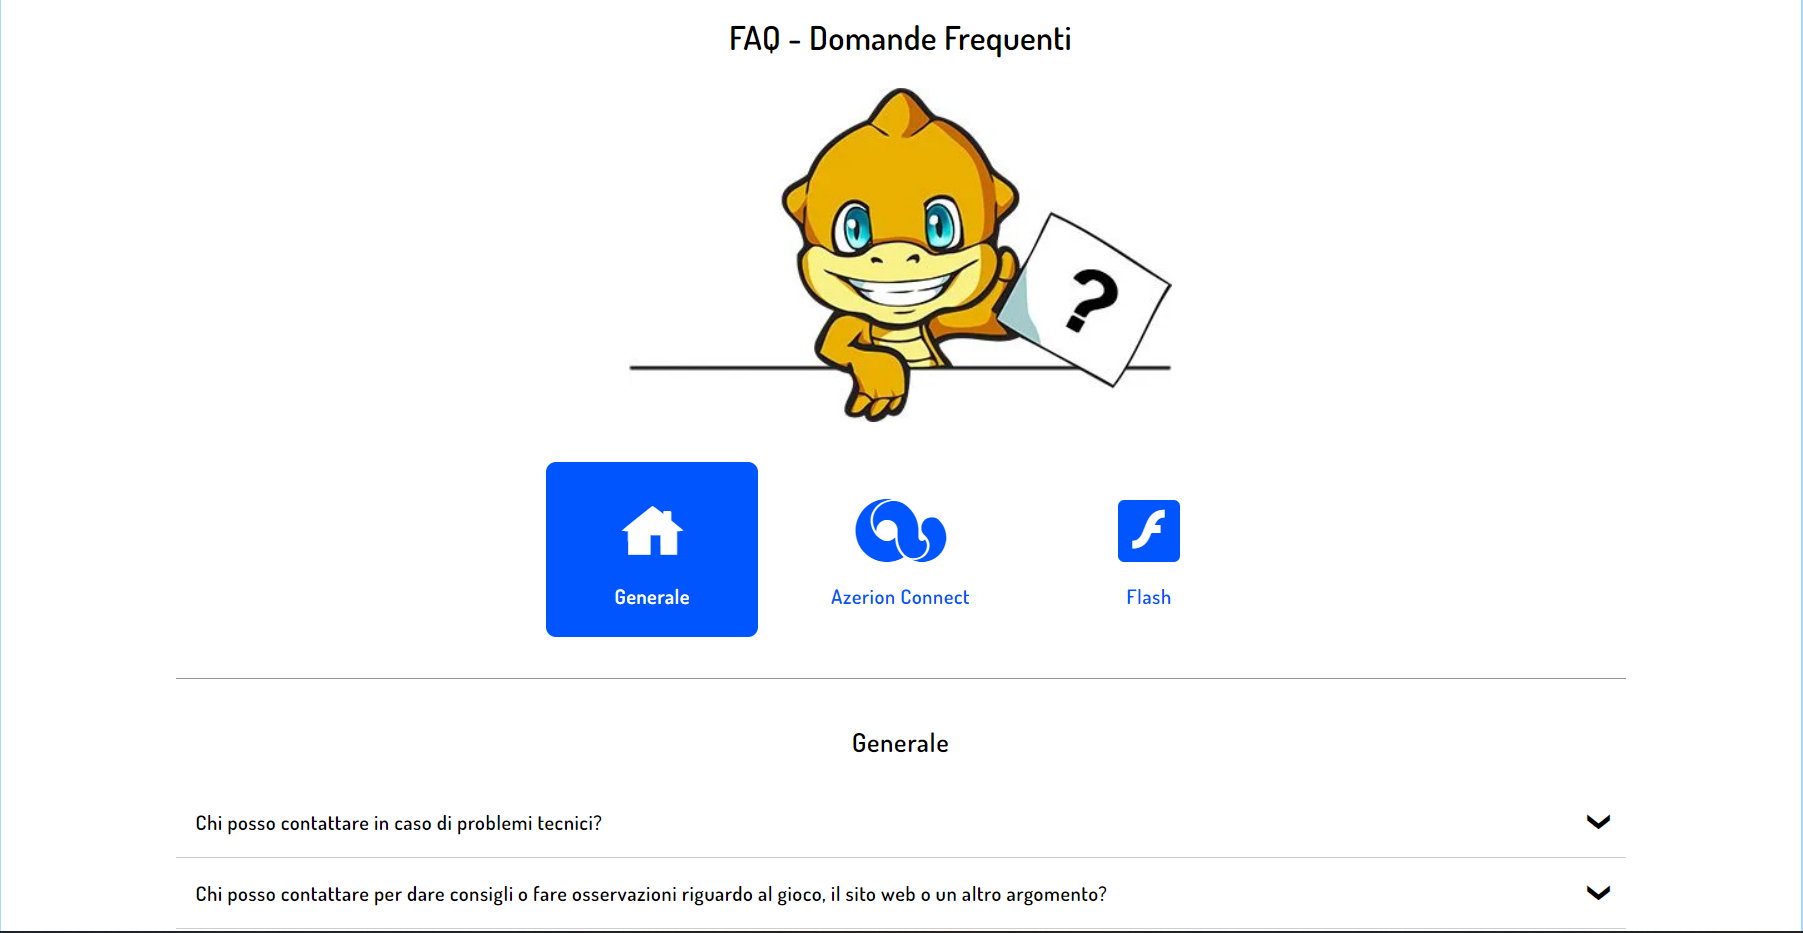
\includegraphics[width=\linewidth]{Assestment21.png}
        \centering
    \end{figure}
    Si può notare come la sezione "Azerion Connect" sia identica per entrambe le sezioni e come sia le FAQ che la sezione di Aiuto, contengano in realtà entrambe delle FAQ. Non ci sono violazioni delle euristiche per quanto riguarda la pagina delle FAQ e dell'Help.


    \subsubsection{Altri Problemi Riscontrati dall’Ispezione}
    Nel banner superiore non sono presenti tutte le categorie e/o un bottone o menù per accedere alla lista delle categorie. Per accedere alla lista di tutte le categorie è necessario accedere alla lista di sotto-categorie di una categoria. 
    Un’altro errore riscontrato è la violazione dell’euristica di coerenza, nell’immmagine rappresentante i giochi preferiti, per i quali una volta viene utilizzata una stella nella schermata di un gioco mentre nel menù viene utilizzato un cuore.

    \begin{figure}[H]
        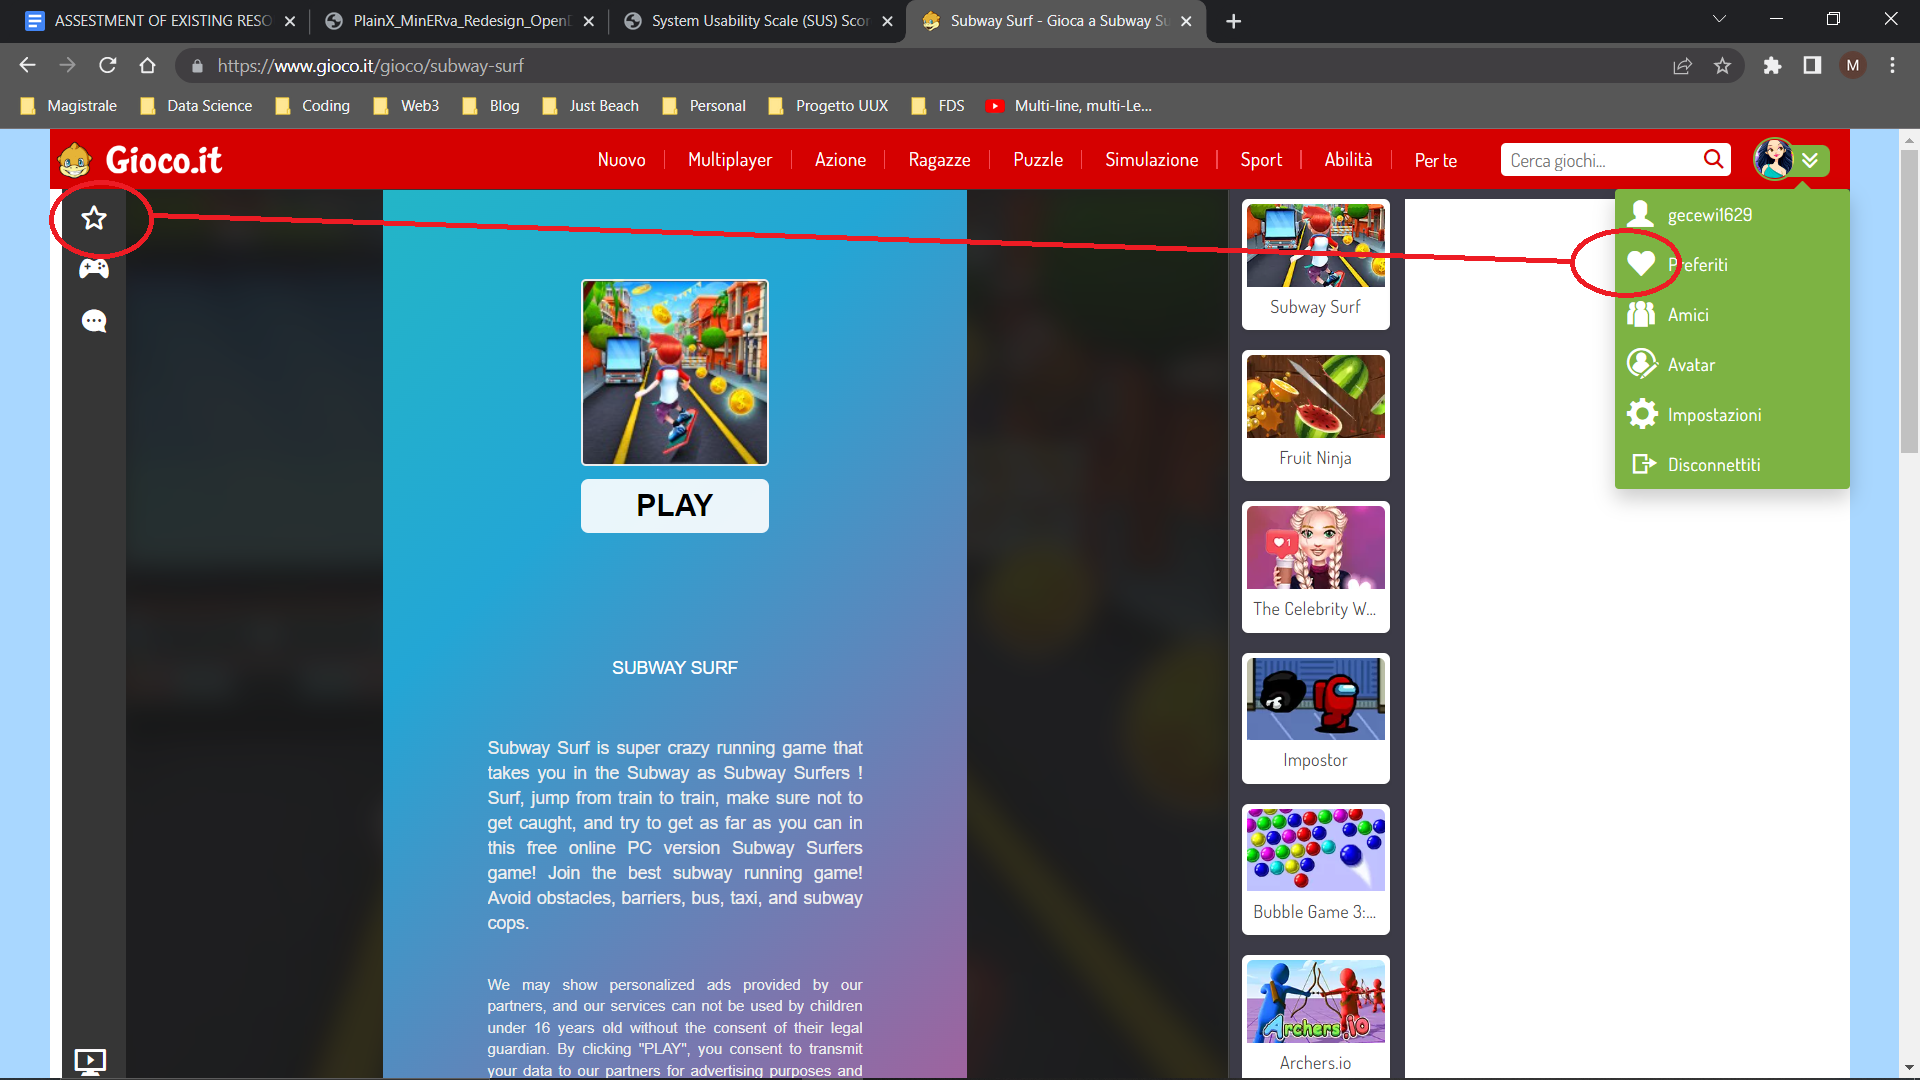
\includegraphics[width=\linewidth]{Assestment18.png}
        \centering
    \end{figure}
    \subsection{Reverse Analysis: Linee guida vs Sistema}
    \subsubsection{Home Page}
    1.\textbf{Gli elementi della home page sono chiaramente focalizzati sui compiti chiave degli utenti (è stata evitata la "featurite") }\\
    La home page è troppo carica consiglia all’utente un numero esagerato di giochi a cui giocare. Inoltre alcune categorie sono nascoste e non accessibili a primo impatto dagli utenti. 

    \subsubsection{Task Orientation}
        1. \textbf{Il sito è libero da informazioni irrilevanti e che possono generare confusione}\\
            Il sito è troppo denso di informazioni, spesso inutili e ripetive. Molti giochi sono doppioni di altri che potrebbero essere accorpati in uno. La sezione profilo è totalmente inutle e non aggiunge nessuna informazione rilevante.  \\
        2. \textbf{Le informazioni vengono presentate in un ordine facile e logico e naturale}\\
        I risultati della ricerca non vengono riportati nè in ordine di rilevanza e popolarità del gioco, nè in ordine alfabetico e non c’è nessun pulsante di ordinamento. Lo stesso vale per la lista di categorie dei giochi. \\
        3. \textbf{Il sito richiede uno scrolling ed un clicking minimale }\\
        La home page non è visibile senza scrolling verticale.\\ 
        10. \textbf{Quando una pagina presenta tante informazioni l’utente può filtrarle.}\\
        L’utente non può filtrare in nessun modo, se non per categorie, i giochi. Anche i risultati della ricerca non sono filtrabili (e neanche ordinabili) in nessun modo.\\
        11. \textbf{Il sito permette agli utenti di customizzare dei parametri di tempo operazionali (tempo di logoff, tempo d’uso ecc)}\\
        Il sito non offre questa possibilità.
    
    \subsubsection{Navigation \& IA}
        5. \textbf{Utenti possono ordinare e filtrare le pagine di categoria}\\In nessun caso gli utenti possono filtrare e ordinare i giochi.


    \subsubsection{Page Layout \& Visual Design}
        9. \textbf{C’è un chiaro punto di inizio visuale in ogni schermata.}\\
        Nella home page data la mancanza di uniformità della griglia gli utenti potrebbero incappare in errori di visualizzazione. Ad esempio pensando che i tre giochi centrali siano una categoria a parte, quando questo non è vero per la sezione gioca ora. \\
        10. \textbf{I pulsanti ed i bottoni mostrano che sono stati cliccati.}\\
        Il pulsante nuovo nella home page mostra di essere stato cliccato ma a differenza degli altri non apre nessuna dialog.\\
        11.\textbf{C’è un buon bilanciamento tra contenuto informativo e spazi vuoti} \\
        Nella home page, nelle pagine di ricerca e in quelle di categoria vengono mostrati troppi giochi, che rendono confusionario e difficile orientarsi.\\ 
        12. \textbf{Il sito è piacevole alla vista.}\\
        Nella home page, nelle pagine di ricerca e in quelle di categoria vengono mostrati troppi giochi, che rendono confusionario e difficile orientarsi. 
        15. \textbf{Il grassetto è usato per riconoscere categorie importanti}\\
        Non sempre il grassetto è usato per le categorie. \\
        16. \textbf{Nelle pagine di contenuto le linee di testo non sono nè troppo lunghe ne troppo corte\\}
        A volte le descrizioni sono molto lunghe e fatte di contenuti inutili.\\
        17. \textbf{Le pagine sono state progettate con una griglia sottostante, con gli oggetti allineati orizzontalmente e verticalmente}\\
        La griglia della home page è asimmetrica.\\
        20. \textbf{Le singole pagine sono prive di informazioni irrilevanti e ingombranti }\\
        Spesso le descrizioni dei giochi contengono informazioni doppie o inutili.
        

    \subsubsection{Ricerca}
    Non sono stati riscontrati nuovi problemi.

    \subsubsection{Help, Feedback And Error Tolerance}

    8.\textbf{La conferma dell’utente è richiesta quando si stanno effettuando delle azioni potenzialmente pericolose come la cancellazione di qualcosa \\
    }    
    Quando si elimina un gioco dai preferiti non viene richiesto nessun messaggio di conferma dell'azione. Viene solo comunicata l'effettivo compimento dell'azione.

    \subsubsection{Le euristiche di Nielsen \& le Euristiche di ambito}
        \textbf{Estetica e design minimalista}\\
        Il design del sito è veramente ricco di elementi che generano confusione e difficoltà di scelta nell’utente.\\ 
        \textbf{Il sito deve correttamente vietare di giocare a determinati giochi ad utenti  registrati che non rispettano il vincolo di età.}\\
        Non rispettato poichè pur creando un account con un’età inferiore a 18 anni è comunque permesso giocare a giochi 18+ come i giochi d’azzardo.

    \section{Testing Utenti}
    \label{section: initial_testing}
    Abbiamo poi testato, per rilevare ulteriori problemi, l’applicativo Gioco.it direttamente con gli utenti. 
    \subsection{Protocollo di testing }
    Prima di tutto elenchiamo quello che è il protocollo del test:\\
    Abbiamo scelto di applicare il metodo del “discount usability testing” per le seguenti ragioni:
    \begin{itemize}
        \item Il budget del progetto è limitato, per cui è impossibile avere un team multidisciplinare di esperti per strutturare test professionali. 
        \item Numero limitato di partecipanti. 
        \item Tempo limitato per l’analisi dei dati.
    \end{itemize}

    La lista dei task che abbiamo chiesto di eseguire agli utenti sono le stesse, per una motivazione molto semplice: in caso di figli troppo piccoli i genitori dovranno riuscire ad utilizzare il sito, svolgendo le varie azioni lasciando al bambino solo il compito di giocare, divertirsi ed imparare. 

    I task che dovranno eseguire saranno:
    \begin{enumerate}
        \item Accedere al proprio profilo tramite delle credenziali fornite da noi
        \item  Ricercare il gioco “Subway Surf”
        \item Metterlo nei preferiti 
        \item Lasciare un commento al gioco e poi eliminarlo 
        \item Modifica la tua foto profilo
        \item Inviare una richiesta di amicizia ad un profilo chiamato “Marco”
        \item Annullare la richiesta di amicizia fatta
        \item Vedere la lista di amici
        \item Aprire la sezione dei giochi preferiti 
        \item Eliminare un gioco dai preferiti 
        \item Cercare il gioco “Fruit Ninja” senza utilizzare la barra di ricerca
        
    \end{enumerate}

    Per quanto riguarda la tipologia di test, abbiamo adottato quella sommativa, in quanto gioco.it è un applicazione web già completa: conseguentemente, il fine del test è la ricerca di eventuali problemi che non sono stati scoperti e risolti dagli sviluppatori, nonchè la verifica del soddisfacimento delle necessità raccolte all’inizio della progettazione, nel nostro caso trattandosi di un redesign la valutazione del soddisfacimento delle euristiche. 
    Sarà quindi informale, poichè noi membri del team saremo presenti al momento dell’esecuzione del test da parte degli utenti e parleremo con loro. Sarà poi sequenziale, poichè gli utenti non eseguiranno il test parallelamente ma lo faranno uno dopo l’altro ed economico poichè non faremo ricorso a degli specialisti come degli psicologi o degli statistici durante l’esecuzione del test ma noi saremo i supervisori del test in qualità di membri del team. 
    Chiederemo inoltre agli utenti di parlare ad alta voce per farci ascoltare i ragionamenti che seguono nell’utilizzo dell’applicativo. Raccoglieremo poi infine tramite delle brevi domande dei pareri sull’applicativo e sulla loro esperienza di utilizzo.

    \subsubsection{Dati Raccolti}
    Raccoglieremo dati relativi a tre metriche in particolare:
    \begin{itemize}
        \item Efficienza (l’utente ha commesso errori o è tornato sui suoi passi)
        \item Successo (l’utente ha completato o meno il task)
        \item Learnability (capacità di acquisire familiarità con il sistema )
        \item Soddisfazione (grado di piacere da parte dell’utente nell’effettuare le operazioni)
    \end{itemize}
    \subsubsection{Utenti testati}
    Prenderemo in considerazione soggetti presi da entrambi i segmenti di utenti trovati.\\
    Ada, donna di 48 anni genitore di una ragazza di 13 anni ed un ragazzo di 22. Ada fa assistenza agli anziani e ha un reddito medio basso. Non è solita utilizzare dei laptop, ma ha una sufficiente conoscenza nell’utilizzo di un computer poichè prima dell largo avvento degli smartphone era solita utilizzare un PC. Usa giornalmente il suo smartphone principalmente per l’utilizzo di social network quali Facebook e Whatsapp per rimanere in contatto con i suoi familiari. E’ autonoma nell’uso degli strumenti che conosce, spesso restia a provare nuove funzionalità o nuove applicazioni.\\
    Emili è una ragazza di 13 anni, iscritta all’ultimo anno della scuola media. Le piace passare il suo tempo libero giocando con le amiche quando è possibile altrimenti è ben felice di restare a casa ad utilizzare il suo laptop. Lo usa principalmente per guardare contenuti su YouTube o giocare. 

    \subsubsection{SUS, System Usability Scale}
    Per la valutazione della soddisfazione abbiamo utilizzato il calcolatore del System Usability Scale reso disponibile al link: https://stuart-cunningham.github.io/sus/. Tuttavia avendo effettuato un numero esiguo di test è stato difficile estrarre delle informazioni statisticamente rilevanti.

    \subsection{Risultati per Ada}
    \begin{table}[H]
        \begin{tabular}{|c|c|p{5cm}|c|}
            \hline
            Task & Successo & Efficacia & Apprendibilità \\
            \hline
            1 & Si & Alta & Alta \\
            \hline
            2 & Si & Medio-Alta (ha cliccato sulla categoria di giochi e non sul gioco direttamente) & Alta \\
            \hline
            3 & Si & Alta & Alta \\
            \hline
            4 & Si & Medio-Alta (durante l'eliminazione ha tentato di usare il tasto dx per poi vedere e usare il menù di opzioni) & Alta \\
            \hline
            5 & Si ma con assistenza & Bassa (l’utente ha dapprima cliccato su impostazioni nella sezione aggiorna dati personali. E’ poi andato su profilo non trovando nulla e trovando sconforto nella visualizzazione di un messaggio di errore. E’ riuscita a completare il task dopo aver ricevuto l’indicazione di usare il tasto avatar.) & Bassa \\
            \hline
            6 & Si & Medio-alta (cercavi nella home una sezione ) & Alta \\
            \hline
            7 & Si & Alta & Alta \\
            \hline
            8 & Si & Alto & Alto \\
            \hline
            9 & Si & Alto & Alto \\
            \hline
            10 & Si & Alto & Alto \\
            \hline
            11 & fallimento & L’utente ha dovuto usare la barra di ricerca pur avendo correttamente cercato tra i giochi di abilità nella sottocategoria giochi con punteggio record. Situazione non ripetibile nel caso in cui non conosca il nome del gioco.  & \\
            \hline
        \end{tabular}
    \end{table}

    \subsection{Risultati per Emili}
    \begin{table}[H]
        \begin{tabular}{|c|c|p{5cm}|p{4cm}|}
            \hline
            Task & Successo & Efficacia & Apprendibilità \\
            \hline
            1 & Si & Alta & Alta \\
            \hline
            2 & Si(con barra di ricerca) & Medio - Alta (ha cliccato sulla categoria di giochi e non sul gioco direttamente) & Alta \\
            \hline
            3 & Si & Alta & Alta \\
            \hline
            4 & Si & Media (tentava di postare il commento schiacciando invio) & Alta \\
            \hline
            5 & Si ma con assistenza & Medio-Bassa
            (non ha usato l’opzione avatar). Ha cercato invano di cliccare sul profilo senza foto per poi capire che non era un bottone cliccabile & Media(Un messaggio di errore sul profilo ha creato confusione)   \\
            \hline
            6 & Si & Alto & Alto \\
            \hline
            7 & Si & Alto & Alto \\
            \hline
            8 & Si & Alto & Alto \\
            \hline
            9 & Si & Alto & Alto \\
            \hline
            10 & Si & Media (Dopo aver correttamente aperto la sezione dei giochi preferiti nel tentativo di eliminare subway surf dai preriti ha erroneamente cliccato il pulsante impostazioni) & Alto \\
            \hline 
            11 & Fallimento & L’utente ha dovuto usare la barra di ricerca. Situazione non ripetibile nel caso in cui non conosca il nome del gioco. & \\
            \hline
        \end{tabular}
    \end{table}
    Mostriamo adesso i risultati del questionario SUS, sia per Ada che per Emili. 
    \begin{table}[H]
        \begin{tabular}{|p{10cm}|c|c|}
            \hline
            \textbf{Domanda} & \textbf{Ada} & \textbf{Emili}\\
            \hline
            1. Credo che utilizzerei il sistema frequentemente & 3 & 4\\
            \hline
            2. Ho trovato il sistema inultimente complesso & 1 & 2 \\
            \hline
            3. Credo che il sistema sia facile da usare & 4 & 4 \\
            \hline
            4. Penso che sia necessario il supporto di una persona tecnica per riuscire ad utilizzare il sistema & 1 & 1 \\
            \hline
            5. Ho trovato le varie funzioni del sistema ben integrare & 2 & 2 \\
            \hline
            6. Credo ci sia troppa inconsistenza nel sistema. & 3 & 1\\
            \hline
            7. Immagino che la maggior parte delle persone impari ad usare il sistema molto velocemente & 4 & 5 \\
            \hline
            8. Ho trovato il sistema molto difficile da usare. & 2 & 2\\
            \hline
            9. Mi sono sentito molto a mio agio ad usare il sistema. & 3 & 3\\
            \hline
            10. Ho dovuto imparare tante cose prima di riuscire ad usare il sistema. & 1 & 2 \\ 
            \hline
            Punteggio SUS & 65, grado D & 75, grado C \\
            \hline
        \end{tabular}
    \end{table}
    \subsection{Analisi dei risultati}
    Si può facilmente notare come nei test eseguiti gli utenti abbiano riscontrate difficoltà simili negli stessi task. 
    \begin{itemize}
        \item Per quanto riguarda il task 2 entrambi gli utenti hanno cliccato sul primo risultato che la ricerca offriva (E1), ma questo allungava di un passaggio il completamento del task poichè si trattava della categoria di giochi e non del gioco in sè. Inoltre Emili in questo caso, capendo l’errore commesso ha manifestato un po’ di dissenso sulla scelta da parte dei progettisti di gioco.it di creare una categoria di giochi di questo tipo. 
        \item Per il task 4 Emili tentava invano di premere invio per inviare il commento come fosse una chat (E2) per poi successivamente capire che bisognava utilizzare il pulsante “Posta”. 
        \item Per il task 5 entrambi gli utenti hanno riscontrato errori più gravi. Entrambi sono rimasti “storditi” da un messaggio di errore 
        %IMMAGINE 20%
        Inoltre gli utenti cercavano invano di modificare l’immagine tramite le impostazioni (E3) o cliccando sull’anteprima dell’avatar (E4). Emili è riuscita dopo un po di esitazioni a trovare il menu avatar, Ada si stava arrendendo e noi membri del team abbiamo indicato il menu avatar per permetterle di concludere il task. Ada ha dichiarato di cercare una pagina o un’impostazione nominata “immagine del profilo”, come su Facebook
        \item Per il task 10 l’errore è stato commesso solo da Emili che però è subito tornata sui suoi passi passando dalla sezione impostazioni (E5) a quella preferiti.
        \item Il task numero 11 è quello che ha causato più problemi. Tutti gli utenti hanno denunciato la mancanza di un opportuno sistema di filtraggio e ordinamento (E6) all’interno del sito oltre che una mancanza di chiara  classificazione e divisione nelle categorie(E7). Un’altro problema riscontrato da Ada è legato al fatto che nonostante avesse cliccato sulla categoria Abilità (quella corretta per il gioco fruit ninja) il menu delle sottocategorie si è aperto nella sezione sbagliata (E8). Inoltre nessuno dei due utenti è riuscito a completare il task, poichè le ricerche per categoria riportano troppi giochi.       
    \end{itemize}
    
    Si è quindi riscontrato una certa difficoltà da parte degli utenti nell’utilizzo dei menù per la modifica e la gestione del profilo e delle informazioni ad esso relative. 
    Gli utenti hanno, inoltre,dichiarato un certo senso di difficoltà nella home page del sito poichè troppo ricca di contenuti.
    \subsection{Lista errori}
    Elenchiamo di seguito quindi tutti gli errori riscontrati, con la loro frequenza e la loro criticità:
    \begin{table}[H]
        \begin{tabular}{|p{8cm}|c|c|}
            \hline
            \textbf{Errore} & \textbf{Frequenza} & \textbf{Classificazione} \\
            \hline
            E1. Il sito attuale propone prima nei risultati le categorie di giochi che il gioco stesso. Gli utenti sono attirati dal cliccare il primo risultato allungando di un passo il path per il task. & 80\% & Cosmetico \\
            \hline
            E2. Non è possibile postare un commento premendo invio invece che il tasto "Posta". & 50\% & Cosmetico \\
            \hline
            E3. Gli utenti cercavano di accedere alla modifica dell'avatar tramite le impostazioni. & 60\% & Cosmetico \\
            \hline
            E4. Gli utenti cercavano di accedere alla modifica dell'avatar cliccando sull'anteprima. & 80\% & Serio \\
            \hline
            E5. Gli utenti accedevano alla sezione impostazioni per eliminare un gioco dai preferiti. & 30\% & Cosmetico \\
            \hline 
            E6. Non è presente un sistema di filtraggio e ordinamento dei contenuti. & 90\% & Catastrofico \\
            \hline 
            E7. Mancanza di coerenza tra categorie e sottocategorie, oltre che nella classificazione dei giochi. & 50\% & Serio. \\
            \hline
            E8. Quando si clicca per accedere a un sottomenù di una categoria quest'ultimo si apre indirizzato ad una categoria sbagliata. & 70\% & Cosmetico. \\
            \hline 
        \end{tabular}
    \end{table}
    \subsubsection{Urgency curves}
    Utilizzando i risultati del test dell'utente, possiamo definire le seguenti curve di urgenza dell'impatto, in cui è quantificato l’impatto in relazione alla frequenza o la persistenza degli errori, individuati dall'utente nella fase di test. La linea rossa, nel grafico, costituisce una soglia fissa: gli errori al di sopra della soglia devono essere corretti il prima possibile.     
    \begin{figure}[H]
        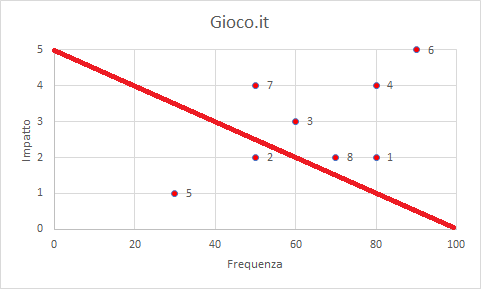
\includegraphics[width=\linewidth]{UrgencyCurve.png}
        \centering
    \end{figure}
\end{document}